

        %%******************************************%%
        %%                                          %%
        %%        Modello di tesi di laurea         %%
        %%            di Andrea Giraldin            %%
        %%                                          %%
        %%             2 novembre 2012              %%
        %%                                          %%
        %%******************************************%%


% I seguenti commenti speciali impostano:
% 1. 
% 2. PDFLaTeX come motore di composizione;
% 3. tesi.tex come documento principale;
% 4. il controllo ortografico italiano per l'editor.

% !TEX encoding = UTF-8
% !TEX TS-program = pdflatex
% !TEX root = tesi.tex
% !TEX spellcheck = it-IT

\documentclass[10pt,                    % corpo del font principale
               a4paper,                 % carta A4
               twoside,                 % impagina per fronte-retro
               openright,               % inizio capitoli a destra
               english,                 
               italian,                 
               ]{book}    

\usepackage[utf8]{inputenc}             % codifica di input; anche [latin1] va bene
                                        % NOTA BENE! va accordata con le preferenze dell'editor

%**************************************************************
% Importazione package
%************************************************************** 

%\usepackage{amsmath,amssymb,amsthm}    % matematica

\usepackage[english, italian]{babel}    % per scrivere in italiano e in inglese;
                                        % l'ultima lingua (l'italiano) risulta predefinita

\usepackage{bookmark}                   % segnalibri

\usepackage{caption}                    % didascalie

\usepackage{chngpage,calc}              % centra il frontespizio

\usepackage{csquotes}                   % gestisce automaticamente i caratteri (")

\usepackage{emptypage}                  % pagine vuote senza testatina e piede di pagina

\usepackage{epigraph}					% per epigrafi

\usepackage{eurosym}                    % simbolo dell'euro

\usepackage[T1]{fontenc}                % codifica dei font:
                                        % NOTA BENE! richiede una distribuzione *completa* di LaTeX

%\usepackage{indentfirst}               % rientra il primo paragrafo di ogni sezione

\usepackage{graphicx}                   % immagini

\usepackage{hyperref}                   % collegamenti ipertestuali

\usepackage[binding=5mm]{layaureo}      % margini ottimizzati per l'A4; rilegatura di 5 mm


\usepackage{microtype}                  % microtipografia

\usepackage{mparhack,fixltx2e,relsize}  % finezze tipografiche

\usepackage{nameref}                    % visualizza nome dei riferimenti                                      

\usepackage[font=small]{quoting}        % citazioni

\usepackage{subfig}                     % sottofigure, sottotabelle

\usepackage[italian]{varioref}          % riferimenti completi della pagina

\usepackage[dvipsnames]{xcolor}         % colori

\usepackage{booktabs}                   % tabelle                                       
\usepackage{tabularx}                   % tabelle di larghezza prefissata                                    
\usepackage{longtable}                  % tabelle su più pagine                                        
\usepackage{ltxtable}                   % tabelle su più pagine e adattabili in larghezza

\usepackage[toc, acronym]{glossaries}   % glossario
                                        % per includerlo nel documento bisogna:
                                        % 1. compilare una prima volta tesi.tex;
                                        % 2. eseguire: makeindex -s tesi.ist -t tesi.glg -o tesi.gls tesi.glo
                                        % 3. eseguire: makeindex -s tesi.ist -t tesi.alg -o tesi.acr tesi.acn
                                        % 4. compilare due volte tesi.tex.

\usepackage[backend=biber,style=verbose-ibid,hyperref,backref]{biblatex}
                                        % eccellente pacchetto per la bibliografia; 
                                        % produce uno stile di citazione autore-anno; 
                                        % lo stile "numeric-comp" produce riferimenti numerici
                                        % per includerlo nel documento bisogna:
                                        % 1. compilare una prima volta tesi.tex;
                                        % 2. eseguire: biber tesi
                                        % 3. compilare ancora tesi.tex.
                                        
\usepackage{xspace}
\usepackage{placeins} % \FloatBarrier per fare il flush delle immagini
\usepackage{sourcecodepro}
\usepackage{listings}
\usepackage{xargs} % Use more than one optional parameter in a new commands
\usepackage[colorinlistoftodos,prependcaption]{todonotes} %todo

%**************************************************************
% file contenente le impostazioni della tesi
%**************************************************************

%**************************************************************
% Frontespizio
%**************************************************************
\newcommand{\myName}{Daniele Marin\xspace}                                    % autore
\newcommand{\myTitle}{Editor visuale per la manipolazione di template HTML}	% titolo tesi         
\newcommand{\myDegree}{Tesi di laurea triennale}                % tipo di tesi
\newcommand{\myUni}{Università degli Studi di Padova}           % università
\newcommand{\myFaculty}{Corso di Laurea in Informatica}         % facoltà
\newcommand{\myDepartment}{Dipartimento di Matematica}          % dipartimento
\newcommand{\myProf}{Claudio Enrico Palazzi\xspace}                                % relatore
\newcommand{\myLocation}{Padova\xspace}                                % dove
\newcommand{\myAA}{2016-2017\xspace}                                   % anno accademico
\newcommand{\myTime}{Giugno 2017\xspace}                                  % quando

\newcommand{\myCompany}{Zucchetti S.p.a.\xspace}

\newcommand{\glossario}[1]{\textit{#1\ped{\ped{G}}}}            % per il glossario



%**************************************************************
% Impostazioni di impaginazione
% see: http://wwwcdf.pd.infn.it/AppuntiLinux/a2547.htm
%**************************************************************

\setlength{\parindent}{14pt}   % larghezza rientro della prima riga
\setlength{\parskip}{0pt}   % distanza tra i paragrafi


%**************************************************************
% Impostazioni di biblatex
%**************************************************************
\bibliography{bibliografia} % database di biblatex 

\defbibheading{bibliography}
{
    %\cleardoublepage
    %\clearpage
    \phantomsection 
    %\addcontentsline{toc}{chapter}{\bibname}
    \addcontentsline{toc}{chapter}{Riferimenti}
    \chapter*{\bibname\markboth{Sitografia}{Sitografia}}
}

\setlength\bibitemsep{1.5\itemsep} % spazio tra entry

\DeclareBibliographyCategory{web}


\defbibheading{web}{\section*{Siti Web di riferimento}}


%**************************************************************
% Impostazioni di caption
%**************************************************************
\captionsetup{
%    tableposition=top,
    figureposition=bottom,
    font=small,
    format=hang,
    labelfont=bf
}

%**************************************************************
% Impostazioni di glossaries
%**************************************************************

%**************************************************************
% Acronimi
%**************************************************************
\renewcommand{\acronymname}{Acronimi e abbreviazioni}

\newacronym[description={\glslink{apig}{Application Program Interface}}]
    {api}{API}{Application Program Interface}
    
\newacronym[description={\glslink{html}{HyperText Markup Language}}]
    {html}{HTML}{HyperText Markup Language}

\newacronym[description={\glslink{rest}{Representational State Transfer}}]
    {rest}{REST}{Representational State Transfer}   

\newacronym[description={\glslink{virtualmachine}{Virtual Machine}}]
    {vm}{VM}{Virtual Machine}   


%**************************************************************
% Glossario
%**************************************************************
\renewcommand{\glossaryname}{Glossario}

\newglossaryentry{Cordova}
{
    name=\glslink{Cordova}{Cordova},
    text=Cordova,
    sort=Cordova,
    description={Apache Cordova è un framework open source per la realizzazione di applicazioni ibride che offre delle API che permettono di accedere via JavaScript ad alcune funzionalità native del dispositivo, come l'accelerometro o la fotocamera}
}

\newglossaryentry{PhoneGap}
{
    name=\glslink{PhoneGap}{PhoneGap},
    text=PhoneGap,
    sort=PhoneGap,
    description={Framework che permette la realizzazione di applicazioni mobile ibride e multi piattaforma utilizzando HTML, CSS e JavaScript. Questo framework è stato pubblicato da Adobe e utilizza Apache Cordova per   interagire con le funzionalità native offerte dai vari sistemi operativi}
}


\newglossaryentry{virtual machine}
{
    name=\glslink{virtual machine}{Virtual machine},
    text=virtual machine,
    sort=virtual machine,
    description={Software che simula delle risorse hardware e che utilizza queste risorse per eseguire determinate applicazione, in modo che queste possano utilizzare le risorse simulate. Le virtual machine hanno vari utilizzi, in questo caso vengono utilizzate per interpretare il codice JavaScript}
}

\newglossaryentry{DOM}
{
    name=\glslink{DOM}{DOM},
    text=DOM,
    sort=DOM,
    description={Il DOM o \textit{Document Object Model} è lo standard del W3C per la rappresentazione ad oggetti di documenti strutturati, come le pagine HTML}
}

\newglossaryentry{WebView}
{
    name=\glslink{WebView}{WebView},
    text=WebView,
    sort=WebView,
    description={Componente grafico offerto dalle API native, sia di iOS, sia di Android, che permette la visualizzazione di pagine HTML}
}

\newglossaryentry{rendering}
{
    name=\glslink{rendering}{Rendering},
    text=rendering,
    sort=rendering,
    description={Termine inglese che indica l'insieme di attività da svolgere per la rappresentazione grafica di un elemento, nel caso specifico dell'interfaccia grafica di un'applicazione}
}

\newglossaryentry{npm}
{
    name=\glslink{npm}{npm},
    text=npm,
    sort=npm,
    description={Acronimo di Node Package Manager, è un sistema di gestione delle dipendenze per le applicazioni JavaScript che permette di installare librerie di terze parti mediante un'interfaccia a riga di comando}
}

\newglossaryentry{riflessione}
{
    name=\glslink{riflessione}{Riflessione},
    text=riflessione,
    sort=riflessione,
    description={In informatica, è la capacità di un programma di analizzare, durante la sua esecuzione, le classi che lo compongono, ricavando così informazioni sulla struttura del proprio codice sorgente}
}
    
\newglossaryentry{gesture}
{
    name=\glslink{gesture}{Gesture},
    text=gesture,
    sort=gesture,
    description={Combinazione di movimenti dell'utente effettuati con le dita su un dispositivo touch-screen, che vengono riconosciuti da un'applicazione}
}

\newglossaryentry{tap}
{
    name=\glslink{tap}{Tap},
    text=tap,
    sort=tap,
    description={Gesture che consiste in un singolo tocco dello schermo da parte dell'utente, è l'equivalente di un click del mouse}
}

\newglossaryentry{pan}
{
    name=\glslink{pan}{Pan},
    text=pan,
    sort=pan,
    description={Gesture che consiste in un tocco prolungato dello schermo da parte dell'utente. Durante l'esecuzione della gesture, l'utente può trascinare il punto di contatto in un modo simile al \textit{drag'n'drop} effettuato con il mouse}
}

\newglossaryentry{swipe}
{
    name=\glslink{swipe}{Swipe},
    text=swipe,
    sort=swipe,
    description={\`E un particolare tipo di pan, effettuato in modo rapito e in una singola direzione, tipicamente da destra verso sinistra o viceversa}
}

\newglossaryentry{pinch-to-zoom}
{
    name=\glslink{pinch-to-zoom}{Pinch-to-zoom},
    text=pinch-to-zoom,
    sort=pinch-to-zoom,
    description={\`E la gesture che viene utilizzata per eseguire lo zoom su un elemento dell'interfaccia grafica, tipicamente un'immagine o una pagina web. Questa gesture consiste nel toccare lo schermo con due dita e allontanarle o avvicinarle tra loro, senza mai staccarle dallo schermo. Nel caso le due dita vengano allontanate viene eseguito uno zoom del contenuto mentre nel caso contrario viene rimpicciolito}
}

\newglossaryentry{singleton}
{
    name=\glslink{singleton}{Singleton},
    text=singleton,
    sort=singleton,
    description={Il singleton è un design pattern individuato dalla \textit{Gang of Four} che ha lo scopo di garantire che venga creata una sola istanza di una determinata classe, e di fornire un punto di accesso globale a tale istanza.
     Nel progetto questo pattern viene implementato sfruttando i moduli CommonJS, creando l'istanza di un oggetto, per poi esportarla come modulo. In questo modo l'oggetto viene creato solo una volta e risulta accessibile a tutta l'applicazione in quanto è un normale modulo CommonJS}
}

\newglossaryentry{proxy}
{
    name=\glslink{proxy}{Proxy},
    text=proxy,
    sort=proxy,
    description={Il proxy è un design pattern individuato dalla \textit{Gang of Four} che prevede l'utilizzo di un classe o oggetto come interfaccia per qualche altro oggetto. Un esempio di utilizzo di questo pattern è dato da Java RMI, che mediante l'utilizzo di oggetti remoti, nasconde la complessità legata al fatto che l'oggetto vero e proprio sul quale viene invocato il metodo si trova su un computer diverso. Nel caso di NativeScript, viene utilizzato un oggetto JavaScript come interfaccia di un oggetto nativo (che può essere sia un oggetto Obj-C, sia Java) in modo che l'oggetto nativo possa essere utilizzato via JavaScript}
}


\newglossaryentry{popover}
{
    name=\glslink{popover}{Popover},
    text=popover,
    sort=popover,
    description={Un popover è un componente delle interfacce grafiche simile ad un pop-up, che compare quanto l'utente seleziona un elemento. A differenza di un pop-up che compare al centro dello schermo, un popover compare vicino al pulsante che l'ha reso visibile ed è collegato ad esse mediante una freccia}
}

\newglossaryentry{API}
{
    name=\glslink{API}{API},
    text=API,
    sort=API,
    description={Indica un'insieme di procedure rese disponibili al programmatore allo scopo di ottenere un'astrazione della complessità della piattaforma sottostante, che può essere sia hardware che software}
}

\newglossaryentry{V8}
{
    name=\glslink{V8}{V8},
    text=V8,
    sort=V8,
    description={V8 è un motore JavaScript open source sviluppato da Google, attualmente incluso in Google Chrome}
}

\newglossaryentry{JavaScriptCore}
{
    name=\glslink{JavaScriptCore}{JavaScriptCore},
    text=JavaScriptCore,
    sort=JavaScriptCore,
    description={JavaScriptCore è un motore JavaScript open source sviluppato da Apple, attualmente incluso in Safari e Safari Mobile}
}

\newglossaryentry{REST}
{
    name=\glslink{REST}{REST},
    text=REST,
    sort=REST,
    description={Riferisce ad un insieme di principi di architetture di rete, i quali delineano come le risorse sono definite e indirizzate. Il termine è spesso usato nel senso di descrivere ogni semplice interfaccia che trasmette dati su HTTP}
}

\newglossaryentry{SDK}
{
name=\glslink{SDK}{SDK},
text=SDK,
sort=SDK,
description={Acronimo di \textit{Software Development Kit}, insieme di strumenti per lo sviluppo e la documentazione di software}
}

\newglossaryentry{Obj-C}
{
    name=\glslink{Obj-C}{Obj-C},
    text=Obj-C,
    sort=Obj-C,
    description={Abbreviazione di Objective-C, un linguaggio di programmazione orientato agli oggetti derivato dal C. Questo linguaggio è stato scelto da Apple come strumento di sviluppo per le applicazione iOS e Mac OS X}
}

\newglossaryentry{MVC}
{
    name=\glslink{MVC}{MVC},
    text=MVC,
    sort=MVC,
    description={Pattern architetturale che prevede la separazione tra la logica di gestione dei dati e come questi dati vengono presentati. Il pattern prevede la divisione dell'architettura in tre parti: \textbf{Model}: si occupa della gestione dei dati; \textbf{View}: si occupa di visualizzare i dati presenti nel model; \textbf{Controller}: si occupa di aggiornare il model in base alle operazioni che l'utente compie sulla view}
}

\newglossaryentry{FPS}
{
name=\glslink{FPS}{FPS},
text=FPS,
sort=FPS,
description={\textit{fotogrammi per secondo}, è un unità di misura utilizzata per indicare la frequenza con la quale vengono generati dei fotogrammi}
}

\newglossaryentry{mock}
{
name=\glslink{mock}{Mock},
text=mock,
sort=mock,
description={Nella programmazione ad oggetti un mock è un particolare tipo di oggetto che simula il comportamento di un oggetto più complesso. Viene utilizzato nei test d'unità per isolare un componente dalle sue dipendenze in modo da poter verificare il corretto funzionamento del componente, senza che questo venga influenzato da eventuali errori presenti nei componenti da cui dipende}
}






 % database di termini
\makeglossaries


%**************************************************************
% Impostazioni di graphicx
%**************************************************************
\graphicspath{{immagini/}} % cartella dove sono riposte le immagini


%**************************************************************
% Impostazioni di hyperref
%**************************************************************
\hypersetup{
    %hyperfootnotes=false,
    %pdfpagelabels,
    %draft,	% = elimina tutti i link (utile per stampe in bianco e nero)
    colorlinks=true,
    linktocpage=true,
    pdfstartpage=1,
    pdfstartview=FitV,
    % decommenta la riga seguente per avere link in nero (per esempio per la stampa in bianco e nero)
    %colorlinks=false, linktocpage=false, pdfborder={0 0 0}, pdfstartpage=1, pdfstartview=FitV,
    breaklinks=true,
    pdfpagemode=UseNone,
    pageanchor=true,
    pdfpagemode=UseOutlines,
    plainpages=false,
    bookmarksnumbered,
    bookmarksopen=true,
    bookmarksopenlevel=1,
    hypertexnames=true,
    pdfhighlight=/O,
    %nesting=true,
    %frenchlinks,
    urlcolor=webbrown,
    linkcolor=RoyalBlue,
    citecolor=webgreen,
    %pagecolor=RoyalBlue,
    %urlcolor=Black, linkcolor=Black, citecolor=Black, %pagecolor=Black,
    pdftitle={\myTitle},
    pdfauthor={\textcopyright\ \myName, \myUni, \myFaculty},
    pdfsubject={},
    pdfkeywords={},
    pdfcreator={pdfLaTeX},
    pdfproducer={LaTeX}
}

%**************************************************************
% Impostazioni di itemize
%**************************************************************
%\renewcommand{\labelitemi}{$\ast$}

\renewcommand{\labelitemi}{$\bullet$}
%\renewcommand{\labelitemii}{$\cdot$}
%\renewcommand{\labelitemiii}{$\diamond$}
%\renewcommand{\labelitemiv}{$\ast$}


%**************************************************************
% Impostazioni di listings
%**************************************************************
% Imposta lo spazio nella list of listing in modo simile alla list of figures/tables
\makeatletter
\let\my@chapter\@chapter
\renewcommand*{\@chapter}{%
  \addtocontents{lol}{\protect\addvspace{10pt}}%
  \my@chapter}
\makeatother


\definecolor{codegreen}{rgb}{0,0.6,0}
\definecolor{codegray}{rgb}{0.5,0.5,0.5}
\definecolor{backcolor}{rgb}{0.98,0.98,0.98}

\renewcommand{\lstlistingname}{Codice}% Listing -> codice
\renewcommand{\lstlistlistingname}{Elenco dei frammenti di codice}% List of Listings -> Frammenti di codice

\lstdefinestyle{mystyle}{
    backgroundcolor=\color{backcolor},   
    commentstyle=\color{Peach}\ttfamily,
    keywordstyle=\color{RoyalBlue},
    numberstyle=\tiny\color{codegray},
    stringstyle=\color{SeaGreen}\ttfamily,
    basicstyle=\footnotesize\ttfamily,
    breakatwhitespace=false,         
    breaklines=true,                 
    captionpos=b,                    
    keepspaces=true,                 
    numbers=left,                    
    numbersep=5pt,                  
    showspaces=false,                
    showstringspaces=false,
    showtabs=false,                  
    tabsize=2,
    frame=trbl, % draw a frame at the top, right, left and bottom of the listing
	frameround=ftff, % angolo in basso a destro curvo
	framesep=4pt, % quarter circle size of the round corners,
	inputencoding=utf8,
    extendedchars=true,
    literate={á}{{\'a}}1 {à}{{\`a}}1 {é}{{\'e}}1 {è}{{\`e}}1 {ù}{{\`u}}1 {ò}{{\`o}}1,
    belowskip=1em,
    aboveskip=1em,
}

 
\lstset{style=mystyle}

\lstdefinelanguage{JavaScript}
{
  % list of keywords
  morekeywords={ true, false, catch, function, break,	new, class, extends, var, require, switch, return, import, if, while, for, this, View, Text, StyleSheet},
  sensitive=false, % keywords are not case-sensitive
  morecomment=[l]{//}, % l is for line comment
  morecomment=[s]{/*}{*/}, % s is for start and end delimiter
  morestring=[b]' % defines that strings are enclosed in double quotes
}

\lstdefinelanguage{JSON}
{
  % list of keywords
  morekeywords={string, boolean, int, Array, Node, Asset, AssetDetail, Filter, FilterItem},
  sensitive=false, % keywords are not case-sensitive
  morecomment=[l]{//}, % l is for line comment
  morecomment=[s]{/*}{*/}, % s is for start and end delimiter
  morestring=[b]" % defines that strings are enclosed in double quotes
}


%**************************************************************
% Impostazioni di xcolor
%**************************************************************
\definecolor{webgreen}{rgb}{0,.5,0}
\definecolor{webbrown}{rgb}{.6,0,0}


%**************************************************************
% Altro
%**************************************************************

\newcommand{\omissis}{[\dots\negthinspace]} % produce [...]

% eccezioni all'algoritmo di sillabazione
\hyphenation
{
    ma-cro-istru-zio-ne
    gi-ral-din
}

\newcommand{\sectionname}{Sezione}
\addto\captionsitalian{\renewcommand{\figurename}{Figura}
                       \renewcommand{\tablename}{Tabella}}

\newcommand{\glsfirstoccur}{\ap{{[g]}}}

\newcommand{\intro}[1]{\emph{\textsf{#1}}}

%**************************************************************
% Environment per ``TODO''
%**************************************************************

\newcommandx{\unsure}[2][1=]{\todo[linecolor=red,backgroundcolor=red!25,bordercolor=red,#1]{#2}}
\newcommandx{\change}[2][1=]{\todo[linecolor=blue,backgroundcolor=blue!25,bordercolor=blue,#1]{#2}}
\newcommandx{\info}[2][1=]{\todo[linecolor=OliveGreen,backgroundcolor=OliveGreen!25,bordercolor=OliveGreen,#1]{#2}}
\newcommandx{\improvement}[2][1=]{\todo[linecolor=Plum,backgroundcolor=Plum!25,bordercolor=Plum,#1]{#2}}
\newcommandx{\thiswillnotshow}[2][1=]{\todo[disable,#1]{#2}}                     % file con le impostazioni personali}
\begin{document}
%**************************************************************
% Materiale iniziale
%**************************************************************
\frontmatter
% !TEX encoding = UTF-8
% !TEX TS-program = pdflatex
% !TEX root = ../tesi.tex
% !TEX spellcheck = it-IT

%**************************************************************
% Frontespizio 
%**************************************************************
\begin{titlepage}

\begin{center}

\begin{LARGE}
\textbf{\myUni}\\
\end{LARGE}

\vspace{10pt}

\begin{Large}
\textsc{\myDepartment}\\
\end{Large}

\vspace{10pt}

\begin{large}
\textsc{\myFaculty}\\
\end{large}

\vspace{30pt}
\begin{figure}[htbp]
\begin{center}

\includegraphics[height=6cm]{logo-unipd}
\end{center}
\end{figure}
\vspace{10pt} 

\begin{LARGE}
\begin{center}
\textbf{\myTitle}\\
\end{center}
\end{LARGE}

\vspace{10pt} 

\begin{large}
\textsl{\myDegree}\\
\end{large}

\vspace{40pt} 

\begin{large}
\begin{flushleft}
\textit{Relatore}\\ 
\vspace{5pt} 
Prof. \myProf
\end{flushleft}

\vspace{0pt} 

\begin{flushright}
\textit{Laureando}\\ 
\vspace{5pt} 
\myName \\
Matr. \myMatr
\end{flushright}
\end{large}

\vspace{40pt}

\line(1, 0){338} \\
\begin{normalsize}
\textsc{Anno Accademico \myAA}
\end{normalsize}

\end{center}
\end{titlepage} 
% !TEX encoding = UTF-8
% !TEX TS-program = pdflatex
% !TEX root = ../tesi.tex
% !TEX spellcheck = it-IT

%**************************************************************
% Colophon
%**************************************************************
\clearpage
\phantomsection
\thispagestyle{empty}

% !TEX encoding = UTF-8
% !TEX TS-program = pdflatex
% !TEX root = ../tesi.tex
% !TEX spellcheck = it-IT

%**************************************************************
% Sommario
%**************************************************************
\cleardoublepage
\phantomsection
\pdfbookmark{Sommario}{Sommario}
\begingroup
\let\clearpage\relax
\let\cleardoublepage\relax
\let\cleardoublepage\relax

\chapter*{Sommario}

Il presente documento descrive il lavoro svolto durante il periodo di stage, della durata di trecentoventi ore, dal laureando \myName presso l'azienda \myCompany.
L'obiettivo di tale attività di stage è l'analisi di varie librerie Javascript per la realizzazione di template HTML, al fine di poter realizzare un editor grafico che permetta la selezione e la modifica dei template per un loro sucessivo inserimento all'interno di pagine HTML.
Inoltre è stato effettuato uno studio sul comportamento dei template in ambito responsive, sulla possibilità di inserire plug-in jQuery all'interno dei template e su di un metodo di caricamento delle librerie controllato in modo di non avere più istanze della stessa libreria se utilizzata da diversi template.
%\vfill
%
%\selectlanguage{english}
%\pdfbookmark{Abstract}{Abstract}
%\chapter*{Abstract}
%
%\selectlanguage{italian}

\endgroup			

\vfill


% !TEX encoding = UTF-8
% !TEX TS-program = pdflatex
% !TEX root = ../tesi.tex
% !TEX spellcheck = it-IT

%**************************************************************
% Ringraziamenti
%**************************************************************
\cleardoublepage
\phantomsection
\pdfbookmark{Ringraziamenti}{ringraziamenti}

%\begin{flushright}{
% \slshape    
% ``Winter is coming''} \\ 
%	\medskip
%    --- Eddard Stark
%\end{flushright}


%\bigskip

\begingroup
\let\clearpage\relax
\let\cleardoublepage\relax
\let\cleardoublepage\relax

\chapter*{Ringraziamenti}

\noindent \textit{Innanzitutto, vorrei ringraziare il relatore della mia tesi, il Prof. \myProf, per l'aiuto fornitomi durante la stesura di questo documento.}\\

\noindent \textit{Un ringraziamento speciale va al Dot. Gregorio Piccoli, che con il suo entusiasmo mi ha permesso di vivere questa bella esperienza.}\\

\noindent \textit{Desidero inoltre ringraziare con affetto i miei genitori, che con il loro sostegno hanno reso possibile il raggiungimento di questo traguardo.}\\

\noindent \textit{Infine, un ringraziare a tutti gli amici e compagni di corso che mi hanno sopportato e sostenuto durante il mio percorso di studi, grazie a loro questi anni rimarranno una bella ed indimenticabile esperienza.}\\

\bigskip

\noindent\textit{\myLocation, \myTime}
\hfill \myName

\endgroup


% !TEX encoding = UTF-8
% !TEX TS-program = pdflatex
% !TEX root = ../tesi.tex
% !TEX spellcheck = it-IT

%**************************************************************
% Indici
%**************************************************************
\cleardoublepage
\pdfbookmark{\contentsname}{tableofcontents}
\setcounter{tocdepth}{2}
\tableofcontents
\markboth{\contentsname}{\contentsname} 
\clearpage

\begingroup 
    \let\clearpage\relax
    \let\cleardoublepage\relax
    \let\cleardoublepage\relax
    %*******************************************************
    % Elenco delle figure
    %*******************************************************    
    \phantomsection
    \pdfbookmark{\listfigurename}{lof}
    \listoffigures
    \raggedbottom

    %\vspace*{8em}

    %*******************************************************
    % Elenco delle tabelle
    %*******************************************************
    \phantomsection
    \pdfbookmark{\listtablename}{lot}
    \listoftables
    \raggedbottom
        
    %\vspace*{8ex}
    
    %*******************************************************
    % Elenco delle porzioni di codice
    %*******************************************************
    \phantomsection
    \pdfbookmark{\listtablename}{loc}
    \lstlistoflistings
     \raggedbottom
    %\vspace*{8ex}
\endgroup

\cleardoublepage

\cleardoublepage

%**************************************************************
% Materiale principale
%**************************************************************
\mainmatter
%\listoftodos[Notes]
% !TEX encoding = UTF-8
% !TEX TS-program = pdflatex
% !TEX root = ../tesi.tex
% !TEX spellcheck = it-IT

%*************************************************************
\chapter{Introduzione}
\label{cap:introduzione}
%*************************************************************

\section{L'azienda}

\begin{figure}[htp]
\centering

\includegraphics[width=\textwidth/2]{../immagini/logo_zucchetti}
\caption{Logo di Zucchetti S.p.a.}
\end{figure}

La \myCompany è una software house con sede a Lodi, che si occupa di soluzioni complete per le aziende, professionisti(commercialisti, consulenti del lavoro, avvocati, curatori fallimentari, notai ecc.) e pubbliche amministrazioni(Comuni, Province, Regioni, Ministeri, società pubbliche ecc.).\\
Il gruppo Zucchetti è la prima azienda italiana in Europa con oltre 3300 addetti, 1100 partner e oltre 105000 clienti.\\
Le soluzioni principali proposte dall'azienda sono :\\
\begin{itemize}
\item Softwere: gestionali, per la sicurezza sul lavoro, analisi business ecc.
\item Hardware: per la rilevazione presenze, controllo accessi e controllo produzione.
\item Servizi: di outsourcing, cloud computing e data center.
\end{itemize}

\subsection{Portal Studio}
Lo stage si è svolto nella sede distaccata di Padova che si occupa di ricerca e sviluppo.
Tra i software che vengono sviluppati in questa sede è presente Portal Studio che consiste in una WEB application per la creazione di siti web.\\
L'applicazione offre all'utente un set completo di strumenti per la creazione di pagine web, permette la creazione e modifica in modo grafico della struttura HTML, la gestione degli stili tramite editor grafico per il CSS ed inoltre permette di gestire i dati provenienti da diversi tipi di database, il loro filtraggio e il binding con varie strutture HTML come liste e tabelle.\\
Il software risulta essere molto maturo e oltre alle funzionalità sopracitate permette anche la creazione di portlet e pagelet e altri elementi riutilizzabili e la gestione di risorse come dati in formato JSON.


\section{Il progetto}
Il progetto proposto dall'azienda per lo stage, nasce dal desiderio di aggiungere all'applicazione Portal Studio una nuova funzionalità che consiste nell'offrire all'utente la possibilità di inserire nelle proprie pagine HTML dei template già pronti e selezionabili da un insieme prestabilito.\\
Questo desiderio ha portato l'azienda ad interessarsi ai template engine come Mustache.js, HandlebarJS ecc.\\
Lo stage si divide in due parti.\\
La prima consisteva nello studio dei template e degli aspetti ad essi correlati, la seconda nella realizzazione di un editor che ne permettesse la visualizzazione e la modifica.\\
Le parti più rilevanti del lavoro svolto sono state sicuramente:
\begin{itemize}
	\item la scelta della libreria da utilizzare nello sviluppo del progetto, che è stata individuata analizzando le caratteristiche di varie librerie per il templateing, cercando fra queste quella che in miglior modo si adeguasse ai requisiti del progetto.
	Questa libreria è stata scelta sapendo che l'azienda l'avrebbe utilizzata per il proprio applicativo quindi i risultati dell'analisi effettuata sono stati discussi con il tutor aziendale;
	
	\item il lavoro di prototipazione relativo ai template, svolto inizialmente per confrontare le potenzialità delle librerie analizzate e in seguito per la creazione dei template necessari per il progetto;
	
	\item l'integrazione di plug-in jQuery all'interno del template, che ha richiesto la valutazione di varie soluzioni che permettessero di ottenere il risultato desiderato;
	
	\item la realizzazione della parte dell'editor relativa alla modifica dei dati, che permette di adattarsi a qualsiasi tipo di template HTML ed SVG e inoltre, nonostante i pochi tipi primitivi forniti da JavaScript, di individuare a quale elemento (immagine, URL, colore, ecc.) si riferiscano i dati dei template.
	  
\end{itemize}
\subsection{Prima parte}
La prima parte del progetto inizia con la realizzazione di qualche template prototipo, utile sia per studiare le possibilità della libreria scelta sia per avere un insieme di template da inserire nell'editor che è stato realizzato in seguito.\\
Durante questa parte del progetto l'attenzione è stata rivolta alla possibilità di realizzare template statici, dinamici, template come composizione di altri template (es. lista di contatti) e template che utilizzano SVG.\\
In seguito alla realizzazione dei template prototipo è stato effettuato uno studio sulla possibilità di rendere i template responsive cioè permetterne la visualizzazione sia su dispositivi desktop che mobile.\\
La prima parte si è conclusa con uno studio sulla possibilità di realizzare template che contenessero al loro interno plug-in jQuery e sulla gestione del caricamento delle librerie necessarie al funzionamento dei template all'interno della pagina HTML.

\subsection{Seconda parte}
La seconda parte del progetto consisteva nella realizzazione di un editor grafico che permettesse all'utente la selezione di un template da una lista prestabilita.
In seguito alla selezione del template desiderato quest'ultimo verrà visualizzato in un box dedicato e tramite un editor, che viene costruito sulla base dei dati editabili del template (i dati sono contenuti in un oggetto JSON che fa parte del template), è possibile vedere il comportamento del template durante la modifica dei suoi dati.	\\
Per determinati template, come quelli considerati composti, l'editor deve dare la possibilità di visualizzare direttamente l'oggetto JSON contenente i dati e permetterne la modifica.\\
Non essendo presente una struttura di back-end proposta dall'applicazione Portal Studio, perché ancora in fase di valutazione, l'editor è stato sviluppato separatamente e l'insieme dei template consiste in un gerarchia di directory contenenti i vari elementi che compongono i template (file HTML, JSON, immagini e librerie) suddivise per categoria.\\
Il caricamento delle risorse viene eseguito tramite chiamate \textit{HTTP GET} request, non essendo presenti delle API fornite dall'azienda.

 %introduzione + azienda           
% !TEX encoding = UTF-8
% !TEX TS-program = pdflatex
% !TEX root = ../tesi.tex
% !TEX spellcheck = it-IT

%**************************************************************
\chapter{Librerie analizzate}
\label{cap:librerie-analizzate}
%**************************************************************
In questo capitolo vengono messe a confronto varie librerie \textit{JavaScript} che permettono la realizzazione di template HTML, ne vengono analizzati i pregi e i difetti per arrivare a descrivere i motivi che hanno portato alla scelta della libreria utilizzata nel progetto.\\
In questa fase sono state prese in esame le principali librerie per il \textit{templating}, con esse sono stati realizzati dei prototipi per testarne le potenzialità e per poter effettuare un confronto fra di esse che non fosse solamente teorico.

\section{Considerazioni generali}
Negli ultimi anni sono nate molte librerie che permettono la creazione di template HTML che hanno portato notevoli vantaggi agli sviluppatori, offrendo loro un nuovo strumento che permette di creare modelli HTML per la rappresentazione dei dati e riutilizzarli all'interno di pagine differenti con una considerevole diminuzione del codice JavaScript e HTML che normalmente viene utilizzato per la modifica de DOM.
Queste librerie si sono evolute velocemente fino ad arrivare a permettere agli sviluppatori di creare intere User interface per applicazioni web, creare componenti riutilizzabili ed in qualche caso offrire funzionalità avanzate come il two-way binding.

\subsection{I template con sintassi mustache}
Le librerie studiate durante lo stage utilizzano tutte questa particolare sintassi, che permette di rappresentare variabili, sezioni, parziali ed altri elementi utili alla creazione del template, tramite l'inserimento di \textit{tag}.\\
Questi particolari \textit{tag} sono caratterizzati dall'utilizzo delle parentesi graffe come delimitatori e questo è il motivo per cui vengono definiti mustaches (baffi in inglese).\\
I tag si presentano nella forma "\{\{I P\}\}" dove I è un simbolo o una stringa ed identifica il tipo di tag, mentre P è un parametro o una chiave appartenente all'oggetto JSON correlato al template.\\
Per l'inserimento di variabili o parziali il \textit{tag} è singolo, mentre per l'inserimento di sezioni, controlli del tipo not-exist ed altri, sono presenti un \textit{tag} di apertura ed uno di chiusura.\\
Per capire meglio il funzionamento che sta alla base di questi template engine è utile fare degli esempi.
\newpage
Questo esempio mostra il rendering di due variabili.
\begin{lstlisting}[language=JavaScript, caption=Esempio di template rappresentante una variabile.]
// oggetto JSON contenente i dati
var dati = { name: "Jon", age: 35};
// template HTML con l'aggiunta del tag mustache
var template = "<h1>Il mio nome è {{name}} e ho {{age}} anni.</h1>";

// il risultato del rendering sarà:

Il mio nome è Jon e ho 35 anni.
\end{lstlisting}
In questo esempio viene definito il template per rappresentare una lista di prodotti.
\begin{lstlisting}[language=JavaScript, caption=Esempio di template rappresentante una sezione.]
// oggetto JSON contenente i dati
var dati = prodotti: [
    						{ name: "pane" },
    						{ name: "pasta" },
    						{ name: "biscotti" }
  					];
  					
// template HTML con l'aggiunta del tag mustache
var template = "<p>Lista della spesa:
					<ul>
						{{#prodotti}}
							<li>{{name}}</li>
						{{/prodotti}}
					</ul>
				</p>";

// il risultato del rendering sarà:

Lista della spesa:
- pane
- pasta
- biscotti
\end{lstlisting}

\newpage

\section{Mustache.js}

\begin{figure}[htp]
	\centering
	
\includegraphics[scale=0.44]{../immagini/mustache_logo_2}
	\caption{Logo  Mustache}
\end{figure}

Mustache può essere considerato come il padre dei template system, è open-source e logic-less e presenta implementazioni per i più famosi linguaggi di programmazione, come Java, Phyton, Ruby, PHP, JavaScript e molti altri.\\
Mustache.js è un implementazione per JavaScript del template system Mustache.\\
La libreria è molto leggera e versatile visto che permette il rendering sia lato server che lato client.\\
Le funzioni offerte sono \textit{render} e \textit{parse}, la prima si occupano di creare la stringa HTML contenente il template renderizzato partendo dai dati JSON e dal template HTML e la seconda è opzionale e permette di preparare il template in modo da velocizzare l'operazione di render.\\
Mustache.js viene definita logic-less perché non presenta nessun tipo di costrutto \textit{if-then-else} e loop come \textit{for} o \textit{do-while}
\subsection{Come funziona}
Il suo funzionamento è molto semplice dato che la libreria offre solamente due metodi.\\
Il metodo principale è \textit{Mustache.render(data, template)} che prendendo in ingresso il template HTML, con gli opportuni \textit{tag} mustache, e i dati tramite oggetto JSON, restituisce una stringa risultato dall'interpolazione dei due elementi.\\
La stringa risultante deve essere inserita all'interno della pagina tramite manipolazione del DOM.\\
Sfortunatamente Mustache.js non offre strumenti per la manipolazione del DOM per cui l'inserimento dovrà essere fatto dal programmatore utilizzando funzioni offerte dallo standard JavaScript o da altre librerie come jQuery.
\subsection{Pregi e difetti}
Uno dei pregi principali è sicuramente la semplicità e la leggerezza della libreria.\\
Inoltre la stesura dei template risulta intuitiva e semplificata dall'assenza di costrutti \textit{if-else} o cicli \textit{for}.\\
Come contro si può citare l'impossibilità di creare funzioni aggiuntive per la gestione dei template, possibilità offerta da altre librerie e la totale mancanza di strumenti per la manipolazione del DOM e dei dati del template che costringe il programmatore ad appoggiarsi ad altre librerie.\\
I template una volta renderizzati sono statici e un cambiamento nei dati non ha effetto sulla loro rappresentazione.

\FloatBarrier
\section{HandlebarsJS}

\begin{figure}[htp]
	\centering
	
\includegraphics[width=\textwidth/2]{../immagini/handlebars_logo}
	\caption{Logo  HandlebarsJS}
\end{figure}

HandlebarsJS è una libreria costruita sopra a Mustache quindi offre tutte le funzionalità di quest'ultimo e aggiunge al normale set di \textit{tag} anche costrutti di controllo come l'espressione \textit{if} e iteratori come \textit{each}.\\
La libreria offre anche un set di metodi globali che permettono al programmatore di effettuare varie operazioni sul template e i suoi dati, in più la possibilità di creare delle funzioni personalizzate che possono essere inserite in uno spazio globale e riutilizzate a piacere su diversi template.\\
Handlebare permette di precompilare il template e offre prestazioni migliori rispetto a Mustache.
\subsection{Come funziona}
Il funzionamento di HandlebarsJS è simile a quello di Mustache, avendo a disposizione l'oggetto JSON contenente i dati e il template, prima si compila il template tramite il metodo \textit{Handlebars.compile(template)}, il risultato della compilazione è una funzione che richiamata passandole come parametro l'oggetto JSON provvede ad interpolare i dati con il template e restituisce una stringa HTML che dovrà essere inserita nella pagina.\\
Anche in questo caso l'inserimento del template nella pagina deve essere fatto utilizzando strumenti esterni alla libreria perché essa non offre funzioni adeguate.

\subsection{Pregi e difetti}
Anche per Handlebars la leggerezza della libreria e la velocità nel rendering è da considerare un pregio.\\
Inoltre la possibilità di sfruttare un set di metodi e di poterne creare di propri risulta un vantaggio rispetto a Mustache.\\
Come Mustache i template una volta creati sono statici e una modifica dei dati non causa un aggiornamento del template che deve essere nuovamente ricompilato.
\newpage
\FloatBarrier
\section{Ractive.js}

\begin{figure}[htp]
	\centering
	
\includegraphics[width=\textwidth/3]{../immagini/ractive_logo2}
	\caption{Logo Ractive.js}
\end{figure}

Ractive.js è una libreria sviluppata al \href{https://www.theguardian.com}{theguardian.com} per creare \textbf{reactive interface} per il web, in modo semplice e efficiente.\\
Questa libreria utilizza la sintassi mustache al pari delle librerie viste in precedenza, quindi un template scritto per funzionare con Mustache.JS o HandlebarsJS può essere utilizzato anche con Ractive.js.\\
Ractive.js arricchisce la sintassi mustache con nuovi strumenti come:
\begin{itemize}
	\item Array index;
	\item Object iterator;
	\item Special e restricted reference;
	\item Espressioni;
	\item Alias.
\end{itemize}
Oltre all'estensione della sintassi mustache, Ractive.js offre un set molto variegato di opzioni e metodi che possono essere utilizzati per modificare sia il DOM del template che i suoi dati,  per l'emissione e la ricezione di segnali e la gestione di animazioni.\\
Tutti questi strumenti permettono la realizzazione di template interattivi e di una certa complessità, cosa che non è possibile fare utilizzando le librerie precedentemente descritte.\\
La libreria è compatibile con tutti i browsers e offre un'ottima compatibilità con SVG e lo standard ES15.\\
I template ottenuti con Ractive.js  offrono un \textit{binding} tra la rappresentazione del template e  il data model, quando i dati vengono modificati la libreria modifica in modo intelligente ed efficiente il DOM del tempalte.

\subsection{Come funziona}
Ractive.js utilizza un approccio differente rispetto alle librerie viste in precedenza.\\
In particolare viene istanziato un oggetto di tipo Ractive che può essere inizializzato implementando varie opzioni tra quelle offerte dalla libreria.\\
Le opzioni principali sono l'oggetto JSON contenente i dati, il template e l'elemento HTML a cui dovrà essere agganciato il template all'interno del DOM.\\
Una volta istanziato l'oggetto viene creata nella \textbf{RAM} una rappresentazione virtuale del DOM (virtual DOM) e viene popolato il model con i dati contenuti nel JSON.\\
In seguito viene renderizzata nel browser la rappresentazione del template interpolato con i dati ad esso relativi.\\
Ia libreria si occupa di creare un legame tra il model e il virtual DOM.\\
Nel momento in cui il model subisce variazioni viene effettuato un confronto tra DOM virtuali e nel caso in cui  venga rilevato un cambiamento la libreria si occupa di modificare il DOM reale in modo intelligente, cioè andando a modificare solamente l'elemento interessato e non tutta la pagina.\\
Questa operazione viene effettuata  nella RAM confrontando la rappresentazione virtuale precedente con quella successiva alla modifica e quindi risulta molto veloce.

\subsection{Pregi e difetti}
I pregi di questa libreria risiedono nel fatto che offre un insieme completo di strumenti che permettono di gestire l'intero ciclo di vita di un template.\\
L'arricchimento degli strumenti relativi alla sintassi mustache permette di inserire nel template campi che possono essere risultato di espressioni ed andare a variare sia i dati rappresentati che elementi del CSS, questo permette di creare template che cambiano dinamicamente in base al variare dei dati anche nell'aspetto grafico.\\
Inoltre la possibilità di creare template che racchiudano HTML, CSS, e comportamento all'interno di un unico file, risulta molto comodo nello sviluppo di quest'ultimi.\\  
Come contro, in relazione alle librerie viste in precedenza si può citare il peso maggiore in termini di risorse e la quantità di tempo necessario ad apprendere il funzionamento della libreria.


%\clearpage
\section{Confronto finale}
Mettendo a confronto le varie librerie si nota che \textit{Mustache.js} e \textit{HandlebarsJS} sono molto simili sia come supporto alla sintassi mustache che come approccio previsto per la creazione dei template.\\
Nel confronto fra le due vince sicuramente \textit{HandlebarsJS} per il fatto che offre qualche strumento in più rispetto a \textit{Mustache.js} e la possibilità  di poter usufruire degli helpers lo rendono più completo e versatile.\\
Ractive.js può essere considerata di una categoria superiore rispetto alle due librerie precedenti sia per il suo approccio nella gestione dei template che per il grande numero di funzionalità offerte, che permette la gestione del template in ogni suo aspetto.\\
Questa libreria può essere utilizzata sia per la creazione di template semplici che molto complessi, inoltre è l'unica delle tre librerie ad offrire la possibilità di rendere interattivi i template tramite il data-binding e la gestione degli eventi.


\FloatBarrier
\section{Libreria scelta}
Non essendo stati stabiliti vincoli sulla creazione dei template,  questi possono essere di diversa complessità, possono essere costruiti con linguaggio HTML o SVG e presentare elementi interattivi.\\ Queste condizioni hanno fatto ricadere la scelta sulla libreria Ractive.js, per le sue caratteristiche che la rendono uno strumento potente e versatile e che non limita le possibilità di sviluppo dei template.
 %Analisi dei framework 
% !TEX encoding = UTF-8
% !TEX TS-program = pdflatex
% !TEX root = ../tesi.tex
% !TEX spellcheck = it-IT

%**************************************************************
\chapter{Strumenti e tecnologie utilizzati}
\label{cap:strumenti-tecnologie}
%**************************************************************
\section{Linguaggi utilizzati}
I template e l'editor creati durante il periodo di stage sono stati sviluppati per poter essere utilizzati all'interno di un browser, quindi i linguaggi utilizzati sono strettamente legati a questo ambiente.\\
Questi linguaggi sono i seguenti:
\begin{itemize}
	\item Il linguaggio HTML è stato utilizzato per creare la struttura dei template e dell'editor;
	\item Il linguaggio SVG è stato utilizzato nella creazione di template contenenti immagini vettoriali.
	\item Il linguaggio CSS è stato utilizzato sia per definire la rappresentazione grafica dei template sia dell'editor;
	\item Il linguaggio JavaScript è stato utilizzato per definire il comportamento dell'editor e per implementare varie funzionalità dei template;
	\item La sintassi mustache è stata utilizzata all'interno dei template, sia  HTML che SVG. 
\end{itemize}

\section{JavaScript ES5}
Il codice JavaScript prodotto durante lo sviluppo del progetto segue gli standard ES5 trattandosi della versione supportata dal JavaScriptCore e compatibile con tutti i browser recenti sia in versione desktop che mobile.\\
La libreria \textit{Ractive.js} offre il supporto ad ES2015 permettendo di utilizzare le \textbf{promise} ed altri elementi che sono stati introdotti nello standard ES6 anche se non supportati dal browser.\\
Nel caso in cui il browser supporti le \textbf{promise}, vengono utilizzate quelle definite nel ES6, altrimenti vengono utilizzate quelle definite dalla libreria che per il momento non supportano \textit{Promise.race} e \textit{Promise.cast}.

\section{Editors}
Per lo svolgimento del progetto poteva essere utilizzato qualsiasi editor di testo ma la scelta è ricaduta su \textit{SublimeText} data la sua versatilità e la sua licenza free.\\
Questo editor riconosce di default i linguaggi  HTML, CSS, e Javascript e offre varie funzionalità come l'auto-completamento del codice, e un set di \textit{bundle} che permettono la stesura del codice in modo automatico tramite l'inserimento di \textit{keyword}.\\
Inoltre \textit{SublimeText} permette l'estensione delle sue funzionalità tramite l'aggiunta di moduli offerti dalla comunità che lo supporta.

\section{Inkscape}
Inkscape è un software per la grafica vettoriale libero e open, disponibile per varie piattaforme.\\
Questo software permette la creazione di immagini vettoriali nel formato SVG (Sclable Vector Graphics) e la loro esportazione in più varianti di questo formato.\\
L'utilizzo di questo strumento è risultato molto utile per la creazione della struttura base di vari template, che in seguito sono stati modificati tramite la sintassi mustache.

\section{Google Chrome Dev Tools}\label{sec:chrome}
Sono un insieme di strumenti offerti da Google agli sviluppatori accessibili all'interno del browser Google Chrome.\\
Questi strumenti risultano molto utili sia nella fase di sviluppo che di testing dell'applicazione perché permettono al programmatore di vedere tutti gli elementi che compongono la pagina, ottenere informazioni sul network, tempi di caricamento delle risorse ed altro.\\
Inoltre è possibile eseguire il codice passo passo tramite il debuger integrato e utilizzare la console per stampare messaggi, tramite \textbf{console.log()} o eseguire metodi.
\section{}

%Flow è uno strumento sviluppato da Facebook che effettua l'analisi statica del codice JavaScript per evidenziare potenziali errori dovuti ad un tipo di dato errato o all'utilizzo di valori \texttt{null}.
 %Strumenti e tecnlogie utilizzati
% !TEX encoding = UTF-8
% !TEX TS-program = pdflatex
% !TEX root = ../tesi.tex
% !TEX spellcheck = it-IT

%**************************************************************
\chapter{I template}\label{cap:template}
In questo capitolo viene descritto il lavoro svolto nella prima parte del progetto, che consiste nella realizzazione dei template, nel spiegare come sono stati resi responsive ed in fine come sia stato possibile inserire \textit{plug-in} JQuery al loro interno.\\
Viene anche trattato l'argomento relativo al loro caricamento all'interno della pagina HTML e la gestione delle librerie.
%**************************************************************
\section{Utilizzo di Ractive.js}
In questa sezione viene descritta più in dettaglio la libreria scelta per svolgere il progetto.
\subsection{L'oggetto Ractive}
Per iniziare ad usare Ractive bisogna innanzitutto creare un istanza dell'oggetto Ractive e passarle le opzioni desiderate tra quelle offerte dalla libreria.\\
Una volta creato l'oggetto questo si occuperà di creare e popolare il proprio registro dati e di creare in memoria una rappresentazione virtuale del template.\\
\begin{lstlisting}[language=JavaScript, caption=Creazione di un oggetto Ractive.]
var ractive = new Ractive({
	el: '#container', // id dell'elemento target nella pagina
	template: '<p>{{greeting}}, {{recipient}}!</p>', // esempio di template
	data: { greeting: 'Hello', recipient: 'world' } // oggetto JavaScript contenente i dati
});
\end{lstlisting}

\newpage

\subsection{Le opzioni principali}
La libreria fornisce un insieme consistente di opzioni che possono essere inizializzate alla creazione dell'oggetto Ractive.\\
Queste si dividono in sei categorie che sono le seguenti:
\begin{itemize}
	\item data;
	\item templating;
	\item transitions;
	\item binding;
	\item parse;
	\item lifecycle event.
\end{itemize}

Tutte queste opzioni opportunamente inizializzate vanno a definire le proprietà ed il comportamento del template nel suo intero ciclo di vita.\\
Le opzioni principali sono:
\begin{itemize}
	\item \textbf{el}: identifica l'elemento target all'interno del browser DOM dove verrà renderizzato il template;
	\item \textbf{template}: rappresenta il template da renderizzare;
	\item \textbf{data}: rappresenta i dati che dovranno essere interpolati con il template;
	\item \textbf{compute}: oggetto che può contenere espressioni o funzioni che verranno ricalcolate al variare del data model;
\end{itemize}

\subsection{Il two-way data biding}
La libreria fornisce la funzionalità di one-way-binding tra i dati contenuti nel data registry e il virtual DOM, cioè al variare del model il virtual DOM e di conseguenza anche la sua rappresentazione nel browser vengono modificate.\\
Oltre a questo tipo di legame, la libreria offre, per elementi di input , il two-way-binding, che permette di modificare il model al variare dei dati nella view e viceversa.
\begin{figure}[htp]
	\centering
	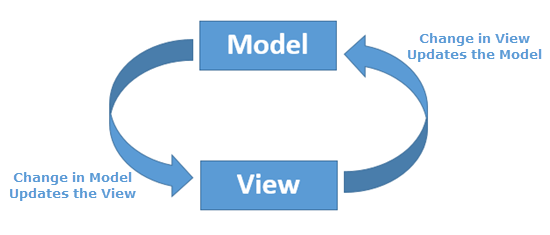
\includegraphics[width=\textwidth/2]{../immagini/twoWayBinding}
	\caption{Rappresentazione two way data binding.}
\end{figure}
\subsection{Gli eventi}
La libreria Ractive implementa il pattern architetturale  \textit{publish/subscribe}, che permette di rispondere o innescare particolari eventi, che attualmente vengono gestiti su due livelli.\\
Il primo è un interazione a basso livello con gli eventi del DOM che viene specificata tramite \textit{directives} del template che specificano anche  come l'evento deve essere gestito, tramite \textit{proxy event} o chiamate a metodi.\\
Il secondo è gestito dalle API \textit{publish/subscribe} e dal sistema di eventi all'interno di Ractive e tra i componenti.\\
I \textit{proxy events} collegano gli eventi del DOM con gli eventi di Ractive, mentre le chiamate a metodi direttamente sull'istanza ractive non utilizzano l'infrastruttura \textit{publish/subscribe}.
\subsection{Il virtual DOM}
Ractive utilizza un sistema differente dagli altri per tracciare le modifiche, ricorrendo al cosiddetto Virtual DOM, ossia a una rappresentazione virtuale della struttura del template immagazzinata in memoria e del tutto simile al DOM originale, del quale può essere vista come una astrazione.\\
Nel momento in cui si verifica un evento ed è necessario “reagire” ad esso modificando gli elementi della pagina, Ractive applica prima tali interventi al Virtual DOM.\\
Attraverso l’analisi delle differenze tra lo stato del Virtual DOM precedente al verificarsi dell’evento e quello nuovo ottenuto dall’applicazione delle modifiche, Ractive determina i cambiamenti effettivi da apportare al DOM vero e proprio.\\
Il calcolo delle differenze tra i due stati del DOM virtuale è estremamente veloce, e grazie a esso si limitano al minimo indispensabile gli interventi sul DOM reale, tendenzialmente più lento, garantendo quindi ottime performance.

\subsection{Plug-in di terze parti}\label{sec:packager}
I \textit{plug-in} permettono di aumentare le funzionalità offerte dalla libreria Ractive.\\
Agli sviluppatori è data la possibilità di creare i propri \textit{plug-in} o di scegliere quelli più adatti alle proprie esigenze da una lista presente sul sito di Ractive.js.\\
Durante lo sviluppo del progetto sono stati utilizzati i \textit{plug-in} \href{https://github.com/ractivejs/ractive-events-tap}{ractive-events-tap}, per gestire il click/tap sui dispositivi mobili , e \href{https://github.com/ractivejs/ractive-load}{ractive-load}, per il caricamento tramite protocollo \textit{http} dei template.   

\section{Sviluppo dei template}
La creazione dei template, per il progetto, non presentava nessuna restrizione né per la forma né per i contenuti, quindi la decisione di quali template sviluppare era a discrezione del programmatore.\\
L'unica richiesta, per questa fase del progetto, è stata quella di avere template sia HTML che SVG.\\
\subsection{Struttura ddei template}
I template HTML sono strutturati come una pagina web, cioè sono formati dal codice HTML per quanto riguarda i contenuti, il codice CSS per la loro rappresentazione grafica e JavaScript per definire il loro comportamento.\\
Il codice HTML rappresentante il template deve essere arricchito tramite la sintassi \textit{mustache} contenenti le variabili, le espressioni e le direttive necessarie al funzionamento del template.\\
Il comportamento del template viene sviluppato tramite gli strumenti offerti dalla libreria Ractive.
La libreria permette di creare un singolo file che contiene al suo interno l'intero template cioè HTML+mustache, CSS e Javascript.\\
Questo risulta molto vantaggioso in termini di quantità di file e organizzazione dei vari template.\\
Ogni template dovrà inoltre avere un file di tipo JSON contenente i dati da visualizzare ed eventuali immagini o librerie necessarie per il suo corretto funzionamento. 

\section{Rendere il template responsive}

\section{Inserimento plug-in jQuery nei template}

\section{Caricamento dei template nelle pagine HTML}

 %I template
% !TEX encoding = UTF-8
% !TEX TS-program = pdflatex
% !TEX root = ../tesi.tex
% !TEX spellcheck = it-IT

%**************************************************************
\chapter{Analisi dei Requisiti}
\label{cap:analisi-dei-requisiti}
In questo capitolo sono contenuti i requisiti dell'applicazione che sono stati individuati durante il progetto.\\
Le linee guida per la creazione dell'applicazione sono state fornite dal tutor e sulla base di esse sono stati individuati i requisiti che in seguito sono stati discussi con il tutor per ottenerne l'approvazione.
%**************************************************************

\section{Applicazione per la modifica dei template}
L'applicazione richiesta per il progetto deve permettere all'utente di visualizzare un insieme di template predefinito, da cui sia possibile selezionare quello desiderato.\\
In seguito alla selezione del template, l'utilizzatore deve poter visualizzare quest'ultimo all'interno di una \textit{view} apposita.\\
In questa fase deve essere fornito all'utente un editor specifico in relazione al template selezionato, che offra la possibilità di visualizzare e modificare i dati forniti di \textit{default} dal template e di vedere all'interno della \textit{view} dedicata il comportamento del template in seguito alla modifica dei dati.\\
L'applicazione deve eseguire all'interno di un browser e deve essere compatibile con i più importanti fra essi (Chrome, Firefox, Opera ed Edge).
\subsection{Visualizzazione lista dei template} \label{subsec:visualizzazione_template}
Questa sezione dell'applicazione è dedicata alla visualizzazione e selezione dei template disponibili.\\
La lista deve essere composta dalle miniature dei template in modo da offrire una prima visione di come viene rappresentato il template.\\
All'utente deve essere permesso di scorrere tutta la lista tramite uno scroll infinito.\\
La lista deve presentare i template per categorie, le seguenti sono quelle individuate durante l'analisi:
\begin{itemize}
	\item template singoli;
	\item template composti;
	\item template singoli contenenti plug-in JQuery;
	\item template composti contenenti plug-in JQuery;
\end{itemize}
I template \textit{singoli} sono dei template la cui costruzione è frutto dell'interpolazione dei dati con un singolo template, mentre quelli \textit{composti} sono template frutto dell'unione di più template.\\
\begin{figure}[htp]
	\centering
	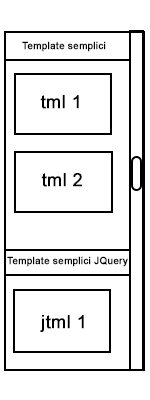
\includegraphics[scale=0.5]{../immagini/mockup_lista}
	\caption{Mockup lista di visualizzazione template.}
\end{figure}

\subsection{Visualizzazione template selezionato}
Questa sezione dell'applicazione è dedicata alla visualizzazione del template selezionato.\\
Il box di visualizzazione non presenta particolari caratteristiche, la sua funzione è quella di mostrare all'utente il template selezionato come verrebbe visualizzato nella pagina html e permettere di osservare i cambiamenti del template in base alla modifica dei dati.
\begin{figure}[htp]
	\centering
	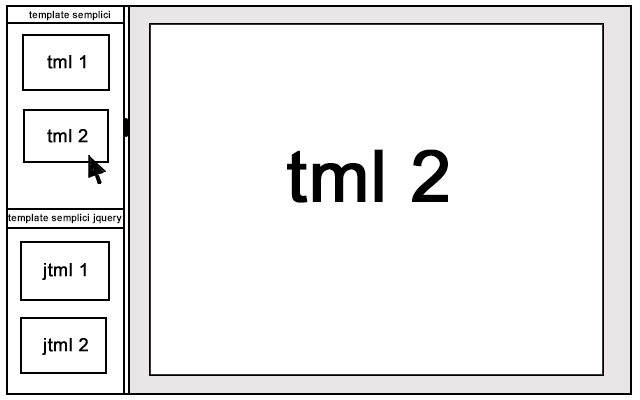
\includegraphics[scale=0.45]{../immagini/mockup_view}
	\caption{Mockup box di visualizzazione template.}
\end{figure}
\subsection{Editor per la modifica del template}
Questa è l'ultima sezione dell'applicazione e si occupa di fornire all'utente gli strumenti per la modifica dei dati relativi al template selezionato.\\
L'utente deve poter visualizzare tutti i dati disponibili per la modifica tramite un interfaccia visuale.\\
Quest'ultima deve fornire all'utente gli strumenti più adeguati per la modifica dei dati in base al loro tipo.\\
Nel caso in cui i template siano composti, l'editor deve visualizzare l'oggetto JSON che rappresenta i dati e dare all'utente la possibilità di modificarne il codice.

%%%%%%%%%%%%%%%%%%%%%%%%%%%%%%%%%%%%%%%%%%%%%%%%%%%%%%%%%%%%%%%%%%%%%%%
%regole per la creazione myminipage
\newenvironment{myminipage}[1]{\minipage{#1} 
	\captionsetup{width=\textwidth, name=Fig., labelfont={it,bf}}
}{\endminipage}
%%%%%%%%%%%%%%%%%%%%%%%%%%%%%%%%%%%%%%%%%%%%%%%%%%%%%%%%%%%%%%%%%%%%%%%
\begin{figure}[htpb] 
	\begin{myminipage}{0.40\textwidth} 
		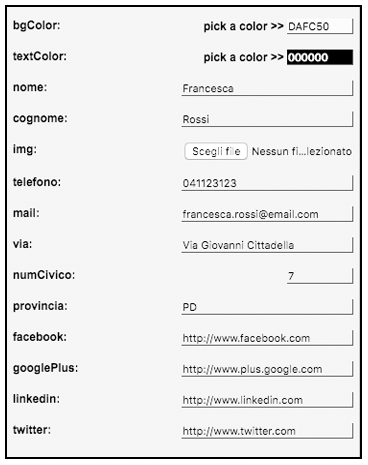
\includegraphics[scale=0.52]{../immagini/mockup_editor1}
		\captionof{figure}{Editor template semplici.}
		%\caption[Prima figura]{Editor template semplici.}\label{fig:1} 
	\end{myminipage} 
	\hspace{0.1\textwidth} 
	\begin{myminipage}{0.40\textwidth}
		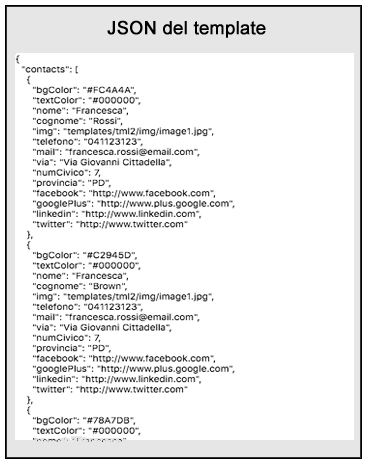
\includegraphics[scale=0.52]{../immagini/mockup_editor2_2}
		\captionof{figure}{Editor template composti.}
		%\caption[Seconda figura]{Editor template composti.}\label{fig:2} 
	\end{myminipage}  
\end{figure}

\newpage
\section{Requisiti individuati}
%parte presa da giacomo
I requisiti individuati sono frutto dall'analisi ed espansione dei requisiti di base e delle discussioni con il tutor aziendale.\\
Di seguito viene descritto il codice con cui sono stati catalogati:
\begin{center}
	\textit{R[T][I][C]}
\end{center}
dove:
\begin{itemize}
	\item \textbf{T}ipo: specifica la tipologia del requisito e può assumere i seguenti valori:
	\begin{itemize}
		\item \textbf{F} - \textit{funzionale}, cioè che determina una funzionalità dell'applicazione;
		\item \textbf{V} - \textit{vincolo}, che riguarda un vincolo che il prodotto deve rispettare.
	\end{itemize}
	\item \textbf{I}mportanza: specifica l'importanza del requisito e può assumere i seguenti valori:
	\begin{itemize}
		\item \textbf{O} - \textit{obbligatorio}, il requisito corrisponde ad un obbiettivo minimo del piano di stage e deve essere soddisfatto per garantire il funzionamento minimo dell'applicazione;
		\item \textbf{D} - \textit{desiderabile}, il requisito corrisponde ad un obbiettivo massimo del piano di stage e deve essere soddisfatto per garantire il funzionamento dell'applicazione;
		\item \textbf{F} - \textit{facoltativo}, indica che il requisito fornisce del valore aggiunto all'applicazione e non era stato previsto nel piano di stage.
	\end{itemize}
	\item \textbf{C}odice: rappresenta un codice che identifica il requisito all'interno di una gerarchia. Questo codice è definito in modo che il requisito \textit{RTIx.y} sia un requisito che va a definire con un grado maggiore di dettaglio alcuni degli aspetti del requisito \textit{RTIx}.
\end{itemize}

%subsection
%\clearpage
\subsection{Requisiti Funzionali}
\normalsize
\begin{longtable}{|l|m{11cm}|}
\hline
\textbf{Id Requisito} & \textbf{Descrizione}\\
\hline
\endhead
RFO1 & L'utente deve poter visualizzare la lista dei template offerti dall'applicazione \\ \hline
RFO1.1 & L'utente deve poter visualizzare le miniature dei template \\ \hline
RFF1.1.1 & La comparsa delle miniature all'interno della lista deve avvenire in modo animato \\ \hline
RFO1.2 & L'utente deve poter scorrere la lista dei template \\ \hline
RFO1.3 & L'utente deve poter visualizzare la categoria dei template \\ \hline
RFO1.4 & L'utente deve poter selezionare i template \\ \hline
RFD1.4.1 & La selezione del template deve avvenire in modo animato \\ \hline
RFO2 & L'utente deve visualizzare il template selezionato in un apposito view-box \\ \hline
RFF2.1 & La comparsa del template nel view-box deve avvenire in modo animato \\ \hline
RFD2.2 & Se il template contiene plug-in JQuery l'utente deve poter visualizzare l'esecuzione del plug-in \\ \hline
RFO2.3 & L'utente deve visualizzare nel view-box l'effetto delle modifiche appotrate al template \\ \hline
RFO2.3.1 & L'utente deve poter visualizzare l'effetto sul template delle modifiche ai dati di tipo colore \\ \hline
RFO2.3.2 & L'utente deve poter visualizzare l'effetto sul template delle modifiche ai dati di tipo numero \\ \hline
RFO2.3.3 & L'utente deve poter visualizzare l'effetto sul template delle modifiche ai dati di tipo booleano \\ \hline
RFO2.3.4 & L'utente deve poter visualizzare l'effetto sul template delle modifiche ai dati di tipo immagine \\ \hline
RFO2.3.5 & L'utente deve poter visualizzare l'effetto sul template delle modifiche ai dati di tipo url \\ \hline
RFO2.3.6 & L'utente deve poter visualizzare l'effetto sul template delle modifiche ai dati di tipo mail\\ \hline
RFO2.3.7 & L'utente deve poter visualizzare l'effetto sul template delle modifiche ai dati di tipo stringa breve\\ \hline
RFO2.3.8 & L'utente deve poter visualizzare l'effetto sul template delle modifiche ai dati di tipo testo \\ \hline
RFO2.3.9 & L'utente deve poter visualizzare l'effetto sul template delle modifiche ai dati di tipo JSON \\ \hline
RFO3 & L'utente deve poter visualizzare i dati di default forniti dal template selezionato \\ \hline
RFO3.1 & L'utente deve poter visualizzare i dati di tipo colore \\ \hline
RFO3.2 & L'utente deve poter visualizzare i dati di tipo numero \\ \hline
RFO3.3 & L'utente deve poter visualizzare i dati di tipo booleano \\ \hline
RFO3.4 & L'utente deve poter visualizzare i dati di tipo immagine \\ \hline
RFO3.5 & L'utente deve poter visualizzare i dati di tipo url \\ \hline
RFO3.6 & L'utente deve poter visualizzare i dati di tipo mail \\ \hline
RFO3.7 & L'utente deve poter visualizzare i dati di tipo stringa breve \\ \hline
RFO3.8 & L'utente deve poter visualizzare i dati di tipo testo \\ \hline
RFO3.9 & L'utente deve poter visualizzare i dati in formato JSON \\ \hline
RFO4 & L'utente deve poter modificare i dati di default forniti dal template selezionato \\ \hline
RFO4.1 & L'utente deve poter modificare i dati di tipo colore \\ \hline
RFD4.1.1 & L'utente deve poter visualizzare il color-picker \\ \hline
RFF4.1.1.1 & La comparsa del color-picker deve avvenire in modo animato \\ \hline
RFF4.1.1.2 & La scomparsa del color-picker deve avvenire in modo animato \\ \hline
RFD4.1.2 & L'utente deve poter selezionare il colore nel color-picker \\ \hline
RFO4.2 & L'utente deve poter modificare i dati di tipo numero \\ \hline
RFO4.3 & L'utente deve poter modificare i dati di tipo booleano \\ \hline
RFO4.4 & L'utente deve poter modificare i dati di tipo immagine \\ \hline
RFD4.4.1 & L'utente deve poter caricare un'immagine da filesystem \\ \hline
RFO4.5 & L'utente deve poter modificare i dati di tipo url \\ \hline
RFO4.6 & L'utente deve poter modificare i dati di tipo mail \\ \hline
RFO4.7 & L'utente deve poter modificare i dati di tipo stringa breve \\ \hline
RFO4.8 & L'utente deve poter modificare i dati di tipo testo \\ \hline
RFO4.9 & L'utente deve poter modificare i dati dell'oggetto in formato JSON \\ \hline
RFD5 & L'utente deve poter visualizzare un messaggio di errore nel caso in cui l'inserimento dei dati avvenga in maniera non corretta \\ \hline

\caption[Requisiti Funzionali]{Requisiti Funzionali}
\label{tabella:req0}
\end{longtable}
\clearpage
\subsection{Requisiti di Vincolo}
\normalsize
\begin{longtable}{|l|m{11cm}|}
\hline
\textbf{Id Requisito} & \textbf{Descrizione} \\
\hline
\endhead
RVO1 & L'applicazione deve utilizzare HTML5 \\ \hline
RVO2 & L'applicazione deve utilizzare CSS3 \\ \hline
RVO3 & L'applicazione deve utilizzare JavaScript \\ \hline
RVO4 & L'applicazione deve utilizzare Ractive.js \\ \hline
RVO5 & L'applicazione deve funzionare su \textit{Google Chrome} versione 52.0 o superiore \\ \hline
RVO6 & L'applicazione deve funzionare su \textit{Firefox} versione 46.0 o superiore \\ \hline
RVD7 & L'applicazione deve funzionare su \textit{Safari} versione 9.0 o superiore \\ \hline
RVD8 & L'applicazione deve funzionare su \textit{Edge} versione 37.0 o superiore \\ \hline
RVD9 & L'applicazione deve funzionare su \textit{Opera} versione 37.0 o superiore \\ \hline
RVF10 & L'applicazione deve funzionare su \textit{Internet Explorer} versione 11.0 o superiore \\ \hline
\caption[Requisiti di Vincolo]{Requisiti di Vincolo}
\label{tabella:req1}
\end{longtable}


\section{Riepilogo requisiti}
I requisiti individuati sono in totale 56 e vengono ripartiti tra le varie tipologie secondo quanto riportato nelle seguenti tabelle.
\\ \\ \\
\begin{minipage}{\textwidth}
	\begin{minipage}[b]{0.49\textwidth}
		\centering
		\begin{tabular}{|l|c|} \hline
			\textbf{Importanza} & \textbf{\#} \\ \hline
			Obbligatori & 42 \\ \hline
			Desiderabili & 9 \\ \hline
			Facoltativi & 5 \\ \hline
			Totale & 56 \\ \hline
		\end{tabular}
		\captionof{table}{Numero di requisiti per importanza}
	\end{minipage}
	\hfill
	\begin{minipage}[b]{0.49\textwidth}
		\centering
		\begin{tabular}{|l|c|} \hline
			\textbf{Tipologia} & \textbf{\#} \\ \hline
			Funzionali & 46 \\ \hline
			Vincolo & 10 \\ \hline
			Totale & 56 \\ \hline
		\end{tabular}
		\captionof{table}{Numero di requisiti per tipologia}
	\end{minipage}
\end{minipage}
\\ \\ \\

\begin{minipage}{\textwidth}
	\begin{minipage}[b]{0.49\textwidth}
		\centering
		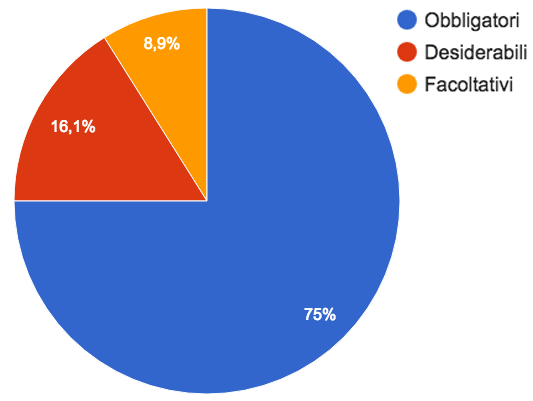
\includegraphics[scale=0.35]{../immagini/chart_requisiti_importanza}
		\captionof{figure}{Requisiti per importanza}
	\end{minipage}
	\hfill
	\begin{minipage}[b]{0.49\textwidth}
		\centering
		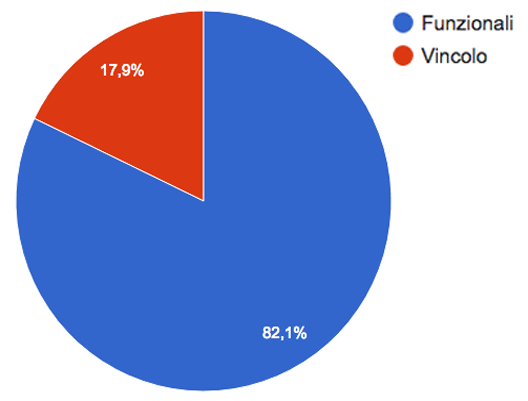
\includegraphics[scale=0.35]{../immagini/chart_requisiti_tipo}
		\captionof{figure}{Requisiti per tipologia}
	\end{minipage}
\end{minipage}
 %Analisi dei requisiti
% !TEX encoding = UTF-8
% !TEX TS-program = pdflatex
% !TEX root = ../tesi.tex
% !TEX spellcheck = it-IT

%**************************************************************
\chapter{Progettazione}
\label{cap:progettazione}
In questo capitolo viene spiegato il metodo di suddivisione delle risorse, come viene effettuato il caricamento dei vari componenti dei template e vengono descritte le funzioni che compongono l'applicazione.
%**************************************************************
\section{Suddivisione template}
Come descritto nel capitolo \textit{Analisi dei requisiti} i template sono stati divisi in quattro tipologie.\\
Dato che non sono presenti delle API fornite dall'azienda, per ottenere informazioni sui template disponibili, come il loro numero, il loro tipo e le risorse che li compongono, è stato deciso di utilizzare un metodo semplice per gestire i template.\\
Questo metodo consiste nel distinguere i vari template tramite il loro nome.\\
Il nome di ogni template è composto da due parti, la prima definisce il tipo e la seconda è un numero che identifica ogni singolo template.\\
Le quattro categorie vengono nominate come segue:
\begin{itemize}
	\item \textbf{tml} identifica i template semplici;
	\item \textbf{jtml} identifica i template semplici contenenti plug-in JQuery;
	\item \textbf{ctml} identifica i template composti;
	\item \textbf{jctml} identifica i template composti contenenti plug-in JQuery.
\end{itemize}
Quindi il nome \textbf{tml1} identificherà il primo dei template semplici all'interno della directory \textit{templates}.\\
I file che definiscono il template utilizzano lo stesso nome del template a cui appartengono.

\section{Caricamento template}
\section{Creazione lista template}
\section{Visualizzazione template selezionato}
\section{Editor per la modifica del template} %Progettazione
% !TEX encoding = UTF-8
% !TEX TS-program = pdflatex
% !TEX root = ../tesi.tex
% !TEX spellcheck = it-IT

%**************************************************************
\chapter{Implementazione}
\label{cap:implementazione}
In questo capitolo vengono descritte le attività svolte durante lo sviluppo dell'applicazione e le principali difficoltà riscontrate.\\
Per lo sviluppo dell'applicazione sono state utilizzate, riadattandole, anche soluzioni sviluppate durante la fase di studio sui template, in particolare quelle relative al caricamento dei template e alla gestione delle librerie jQuery.\\
Durante questa fase il lavoro svolto è stato proposto al tutor aziendale in più riprese perché ne verificasse il comportamento e proponesse eventuali modifiche.
%**************************************************************

\section{Il caricamento dei template}
Il caricamento dei template consiste in tre fasi, che sono:
\begin{itemize}
	\item caricamento delle risorse;
	\item creazione istanza \textit{Ractive};
	\item rendering del template all'interno di un elemento HTML.
\end{itemize}
Per effettuare il caricamento delle risorse sono stati utilizzati due metodi differenti in base al tipo di file da caricare.\\
Il caricamento degli oggetti di tipo JSON, come i dati e l'elenco delle librerie jQuery del template, è stato effettuato tramite un metodo offerto dalla libreria jQuery, che permette di effettuare una \textit{GET HTTP request} per il caricamento specifico di oggetti JSON.\\
Il metodo in questione è \href{http://api.jquery.com/jquery.getjson/}{\texttt{JQuery.getJSON()}} che effettua una \textit{callback} ad un URL e ritorna l'oggetto desiderato.\\
Per effettuare il caricamento del template mustache invece, la comunità di Ractive offre un plug-in chiamato \texttt{ractive-load}\footnote{\url{https://github.com/ractivejs/ractive-load}} che aggiunge un metodo statico alla libreria e permette, tramite la  \textit{promise}\footnote{\url{http://www.ecma-international.org/ecma-262/6.0/\#sec-promise-objects}} \texttt{Ractive.load()} di effettuare il caricamento del file contenente la definizione del template utilizzando \textit{GET HTTP request}.
\newpage
\begin{lstlisting}[language=JavaScript, caption=Chiamate \textit{GET HTTP} per il caricamento delle risorse.]
// carico i dati del template
$.getJSON(dataUrl, function(dati) { // se il caricamento ha successo
	// carico il template tramite Ractive.load
	Ractive.load(tmlUrl).then( function(Template) {
		// creo l'oggetto ractive
		var ractive = new Template({
			el: tmlAnchor,
			data: dati
		});
	...

	});
})
.fail( function() { // errore caricamento, file non valido
	console.log('file non trovato o errore di caricamento!');
});
\end{lstlisting}
Le richieste vengono eseguite in modo asincrono, quindi solamente l'esito positivo della prima \textit{callback} permette l'esecuzione della chiamata a \texttt{Ractive.load()} e l'eventuale istanziazione dell'oggetto \textit{Ractive}.\\
Per quanto riguarda il caricamento di template contenenti plug-in jQuery, il metodo è identico, ma prima di caricare i dati ed il template devono essere caricate le librerie.\\
Il caricamento delle librerie viene effettuato tramite \texttt{JQuery.getJSON()} del file contenente la lista delle librerie e aggiungendo le URL di quest'ultime all'\texttt{header} dell'applicazione tramite la creazione di un tag \texttt{script} per ogni libreria individuata.\\
\begin{lstlisting}[language=JavaScript, caption=Codice per l'aggiunta delle librerie più esempio di JSON e risultato ottenuto.]
// carico le librerie del template
$.getJSON(libsUrl, function(libs) { // se il caricamento ha successo
	// aggiungo le librerie alla pagina HTML
	scriptControll.loadLibs(libs);

	// carico i dati del template
	$.getJSON(dataUrl, function(dati) { // se il caricamento ha successo
		...
		// istanziazione oggetto ractive
})
.fail( function() { // librerie non trovate o errore di caricamento
	console.log('file non trovato o errore di caricamento!');
///////////////////////////////////////////////////////////////////////
// esempio oggetto JSON contenente le URL delle librerie
{
	"libs": [
		"templates/jtml1/lib/actuate-animate.min.js",
		"templates/jtml1/lib/jquery.drawsvg.min.js"
	]
}
///////////////////////////////////////////////////////////////////////
// esempio di risultato prodotto nell'HTML
<head>
		...
	<!-- script aggiunti -->
	<script src="templates/jtml1/lib/actuate-animate.min.js"></script>
	<script src="templates/jtml1/lib/jquery.drawsvg.min.js"></script>
</head>

\end{lstlisting}
Per i template con plug-in jQuery il problema principale è che il template venga renderizzato prima del caricamento delle librerie, questo comporta il non riconoscimento delle funzioni che si riferiscono al plug-in rendendo il template incompleto.\\
Quindi il caricamento delle librerie viene eseguito sempre prima di caricare gli altri elementi del template.\\
Nonostante questa accortezza risulta impossibile verificare l'effettivo caricamento da parte del \textit{browser} delle librerie perché esso viene effettuato in modo asincrono.\\
Questo problema può essere risolto in maniera semplice con un \textit{reload} della pagina o come è stato fatto in un fork dell'applicazione tramite un \textit{preload} di tutte le librerie, che però risulta una soluzione molto onerosa e in certi casi non risolve il problema.

\subsection{Controllo delle librerie caricate}
Uno dei problemi che è sorto durante lo sviluppo in relazione al caricamento delle librerie per i template con plug-in jQuery, è quello di effettuare il caricamento di una o più librerie già caricate in precedenza.\\
Questo comporta la manipolazione inutile del \textit{DOM}, quindi una quantità maggiore di carico per il \textit{browser}.\\
Il problema è stato risolto effettuando un controllo tramite l'implementazione della funzione \texttt{confrontaScript()} che utilizza il metodo \texttt{document.scripts} per ricavare la lista delle librerie caricate dall'applicazione e tramite un confronto con essa decide se sia necessario aggiungere la nuova libreria o meno.\\
Questa funzione viene invocata dalla funzione \texttt{addLibraryFromUrl()} per ogni URL presente nel JSON, ogni qual volta venga caricato un template contenente plug-in.
\begin{lstlisting}[language= JavaScript, caption= Funzione che gestisce il caricamento di una libreria.]
confrontaScript(library) {
	var scriptArray = document.scripts; // array degli script caricati
	var trovato = false;
	for (var i = 0; i < scriptArray.length && !trovato; i++) {
		var scriptUrl = scriptArray[i].attributes.src.value;
		var scriptName = scriptUrl.slice( scriptUrl.lastIndexOf('/')+1, scriptUrl.length);
		if (scriptName === library) {
			trovato = true;
			//console.log('lo script '+library+' è già presente!');
		}
	}
	return trovato;
}

\end{lstlisting}

\section{Visualizzatore lista template}
Dopo aver sviluppato le funzioni per il caricamento dei template è iniziata la fase di realizzazione della sezione adibita alla visualizzazione della lista dei template disponibili.\\
Il problema che si è presentato prima di iniziare lo sviluppo è stato quello di scegliere quali elementi utilizzare per creare la lista.\\
La scelta più adeguata in questo caso sarebbe stata quella di caricare una lista di \textit{thumbnail} (miniature) rappresentanti i vari template disponibili.\\
Questa decisione però, pur essendo la più efficiente, è stata scartata perché avrebbe richiesto la creazione di tutte le miniature e l'aggiornamento delle directory dei template.\\
Per questioni di tempo è stato deciso di caricare direttamente i template nella lista, visto che l'efficienza non era uno dei requisiti importanti per il tutor.\\
Dopo aver discusso il problema e definito il modo di procedere è iniziato lo sviluppo di questa sezione dell'applicazione.\\
La costruzione della lista viene effettuata creando i vari elementi che la compongono in modo sequenziale e inserendoli all'interno elemento HTML predisposto a contenerli.\\
Questa operazione viene effettuata dalle funzioni \texttt{createTemplateList()}, che tramite l'oggetto \hyperref[ttlObject]{\texttt{templatesToLoad}} si occupa di suddividere la lista fra le varie tipologie di template, e \texttt{loadTemplateList()}, che crea l'elemento \texttt{<li>} dedicato a contenere il template.\\
Il rendering viene effettuato all'interno dell'elemento \texttt{<li>} creato in precedenza utilizzando il suo id (creato in maniera univoca) come parametro di ancoraggio per l'oggetto \textit{Ractive} rappresentante il template.
\begin{lstlisting}[language=JavaScript, caption=Implementazione \texttt{loadTemplateList().}]
function loadTemplateList(type, num) {
	// per ogni tipo di template li carico tutti
	for (var i = 1; i < num+1; i++) {
		// creo list item ancora
		var listItem = "<li class='tml-list-item' ><div class='tml-list-item-div'><a class='tml-list-item-a' onclick='selectTml(this)' href='javascript:void(0)' id='"+type+i+"'></a></div></li>";
		// appendo l'elemento alla lista
		$('#tml-list').append(listItem);

		var anchor = '#'+type+i;
		// creo l'oggetto ractive col template relativo
		if (type === 'tml' || type === 'ctml') { // template senza jQuery
			var html = 'templates/'+type+i+'/'+type+i+'.html';
			var dati = 'templates/'+type+i+'/'+type+i+'.json';
			// carico il template
			tl.loadTemplateWithoutJQuery(html, dati, anchor);
		}
		else if (type === 'jtml' || type === 'jctml') { // template senza jQuery
			var html = 'templates/'+type+i+'/'+type+i+'.html';
			var dati = 'templates/'+type+i+'/'+type+i+'.json';
			var libs = 'templates/'+type+i+'/'+type+i+'_libs.json';
			// carico il template
			tl.loadTemplateWithJQueryPlugins(html, dati, libs, anchor);
		}

	}
}
\end{lstlisting}
\section{Visualizzatore template selezionato}
In questa fase di sviluppo è stata realizzata la \textit{view} dedicata alla visualizzazione del template selezionato.\\
Per effettua la visualizzazione è stato necessario:
\begin{itemize}
	\item individuare il template selezionato all'interno della lista;
	\item create un'istanza \textit{Ractive} che lo rappresenti;
	\item renderizzare il template all'interno della \textit{view}.
\end{itemize}
Per individuare il template selezionato è stato implementato l'evento \texttt{onclick} dei vari elementi appartenenti alla lista in modo che richiamino la funzione \texttt{selectTml()} passandogli il riferimento all'elemento che ha lanciato l'evento.\\
Dal riferimento è possibile risalire al nome del template da visualizzare e quindi creare un oggetto \textit{Ractive} che verrà renderizzato all'interno della \textit{view}.\\
Nel momento in cui viene visualizzato il template, viene richiamata la funzione che si occupa della costruzione del relativo editor, il cui sviluppo verrà descritto nella sezione seguente.
\begin{lstlisting}[language=HTML, caption=Chiamata di \texttt{selectTml()} all'evento \texttt{onclick} del list item.]
<li class='tml-list-item' >
	<div class='tml-list-item-div'>
		<a class='tml-list-item-a' onclick='selectTml(this)' href='javascript:void(0)' id='"+type+i+"'></a>
	</div>
</li>
\end{lstlisting}
Le modifiche ai dati sono visualizzate in tempo reale poiché la libreria \textit{Ractive.js} si occupa di effettuare l'update del render in maniera automatica.

\section{Editor per la manipolazione del template}
La realizzazione dell'editor per la modifica dei dati conclude la fase di sviluppo.\\
L'applicazione deve fornire un editor adeguato ad ogni possibile template, quindi risulta necessario individuare i dati modificabili del template e il loro tipo per poter fornire gli strumenti adeguati per la loro modifica.\\
Durante questa fase sono state individuate varie soluzioni per risolvere questo problema.\\
Una di queste consisteva nell'effettuare il parsing del \textit{DOM} del template, individuando il tipo del dato da modificare in base al \textit{tag} HTML che lo conteneva.\\
Questa soluzione è stata scartata perché troppo onerosa da implementare e perché certi dati all'interno del template potevano essere frutto di espressioni o di funzioni implementate nella logica del template, fatto non deducibile da un parsing del \textit{DOM}.\\
La soluzione individuata consiste nell'effettuare il parsing dell'oggetto JSON contenente i dati del template, questo offre la sicurezza sulla quantità di dati modificabili, ma fa sorgere un'altro problema.\\
Il problema riscontrato consiste nel non poter rilevare vari tipi tra quelli descritti nella sezione \textit{Analisi dei requisiti}, come, per esempio i tipi \texttt{colore}, \texttt{immagine}, \texttt{URL}, perché non presenti fra i tipi primitivi in un oggetto JSON.\\
\subsection{Creazione dell'editor}
La realizzazione dell'editor viene effettuata dalla funzione \texttt{creaTml()} che, in base al tipo di template, decide se creare un editor per template semplici o composti.\\
Per template composti è stata implementata la funzione \texttt{creaEditorFullJson()} che si occupa di creare una \textit{text-area} contenente l'oggetto JSON e ne permette la modifica direttamente da codice.\\
Lo sviluppo dell'editor per i template semplici, che viene effettuato dalla funzione \texttt{creaEditor()}, è stato più complesso perché ha richiesto l'individuazione del tipo di ogni dato presente nel JSON e la creazione del relativo strumento.\\
Per effettuare la creazione dei vari strumenti e per individuare i tipi di dato è stata sviluppata la funzione \texttt{parse()} che, in modo ricorsivo, effettua il parse dell'oggetto JSON individuando il tipo dei dati e costruendo per ognuno di essi il relativo strumento di input.\\
Il problema della rilevazione dei tipi non primitivi è stato risolto tramite il confronto dei dati di tipo \texttt{string} con espressioni regolari che rappresentano i seguenti tipi:
\begin{itemize}
	\item \textbf{colore}, rappresentato sia in formato \textit{rgb} che esadecimale;
	\item \textbf{URL}, rappresentato come url generica a risorse web non di tipo immagine;
	\item \textbf{mail}, rappresentato come indirizzo di posta elettronica;
	\item \textbf{immagine}, rappresentato come url a risorse di tipo immagine nei formati \textit{jpg, jpeg, png, gif} e \textit{svg}.
\end{itemize}
Nel caso in cui il tipo rilevato sia un immagine viene costruito un input di tipo \textit{input-file} che permette il caricamento di un immagine da file-system.\\
Mentre per il tipo \textbf{colore} è stato utilizzato il plug-in jQuery \href{http://jscolor.com/}{jscolor}, che permette di visualizzare il colore e propone un utile \textit{color-picker} per effettuarne la modifica.\\
\begin{figure}[htp]
	\centering
	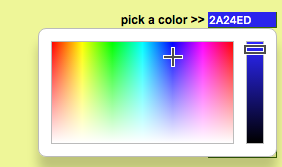
\includegraphics[scale=1]{../immagini/color_picker}
	\caption{Color-picker per la modifica dei tipi colore.}
\end{figure}
\newpage
Per la modifica degli altri tipi vengono utilizzati gli strumenti di input forniti dal linguaggio HTML senza ricorrere a librerie esterne.\\
In seguito viene proposto un estratto della funzione \texttt{parse()}.
\begin{lstlisting}[language=JavaScript, caption=Estratto della funzione \texttt{parse()}]
function parse(obj, el, index, regExpArray, path ){

	if (obj == null || obj == undefined) {
		return;
	}
	else {

	for (var k in obj) {

		if (typeof obj[k] === 'string') { // se è una stringa
			// controllo tramite regExp il tipo della stringa
			
			...

			if (pos === 0) { // è una e-mail
				label = "<label class='json-label'>"+k+": <input type='text' class='json-data-email edit' id='"+path+k+"' value='"+obj[k]+"' ></label><br>";
			}
			else if (pos === 1) { // è una URL
			
				if ( regExpArray[4].test(obj[k]) ) { // se true è un'immagine
					label = "<label class='json-label'>"+k+": <input type='file' class='json-data-img edit' id='"+path+k+"' ></label><br>";
				}
				else {
					label = "<label class='json-label'>"+k+": <input type='text' class='json-data-url edit' id='"+path+k+"' value='"+obj[k]+"' ></label><br>";
				}  
			}
			else if (pos === 2 || pos === 3) { // è un colore
				label =  "<label class='json-label'>"+k+": <span class='pick-color'>pick a color >> <input class='json-data-color jscolor edit' id='"+path+k+"' value='"+obj[k]+"'></span></label><br>";
			}
			else{ // è una normale stringa
				// costruzione input-text o text-area
				...
			}
		}

		else if (typeof obj[k] === 'number') { // se è una numero
			var label = "<label class='json-label'>"+k+": <input type='number' class='json-data-number edit' id='"+path+k+"' value='"+obj[k]+"' ></label><br>";
			$(el).append(label);
		
		}
		
		...
		
		// individuazione altri tipi e ricorsione per Array e Object
		
		...
	}
}
\end{lstlisting}

\subsection{Modifica dei dati}
La funzione \texttt{creaTml()} oltre ad occuparsi di creare l'editor giusto per ogni template, si occupa di aggiornare i dati in seguito a una modifica.\\
La modifica del model del template selezionato avviene tramite l'utilizzo del metodo \texttt{Ractive.set()}, offerto dalla libreria \textit{Ractive.js}.\\
Questo metodo modifica il model ed in seguito lancia l'evento \textit{update} che comporta il re-rendering del template nella pagina, permettendo la visualizzazione delle modifiche in tempo reale.\\

\subsection{Controllo degli input}
Prima di invocare la modifica di un dato viene effettuato un controllo sul dato inserito per verificarne la conformità con il tipo richiesto.\\
Per quanto riguarda i tipi non primitivi, citati in precedenza, vengono utilizzate le espressioni regolari per effettuare il controllo.\\
Nel caso in cui i dati inseriti non siano corretti viene visualizzato un messaggio di errore tramite un \textit{alert-box}. %Realizzazione
% !TEX encoding = UTF-8
% !TEX TS-program = pdflatex
% !TEX root = ../tesi.tex
% !TEX spellcheck = it-IT

%**************************************************************
\chapter{Conclusioni}
\label{cap:conclusioni}
%**************************************************************

Questo capitolo finale espone le conclusioni tratte riguardo alle attività svolte durante il periodo di stage.

\section{Valutazione del risultato e di Ractive.js}
\begin{figure}[htp]
	\centering
	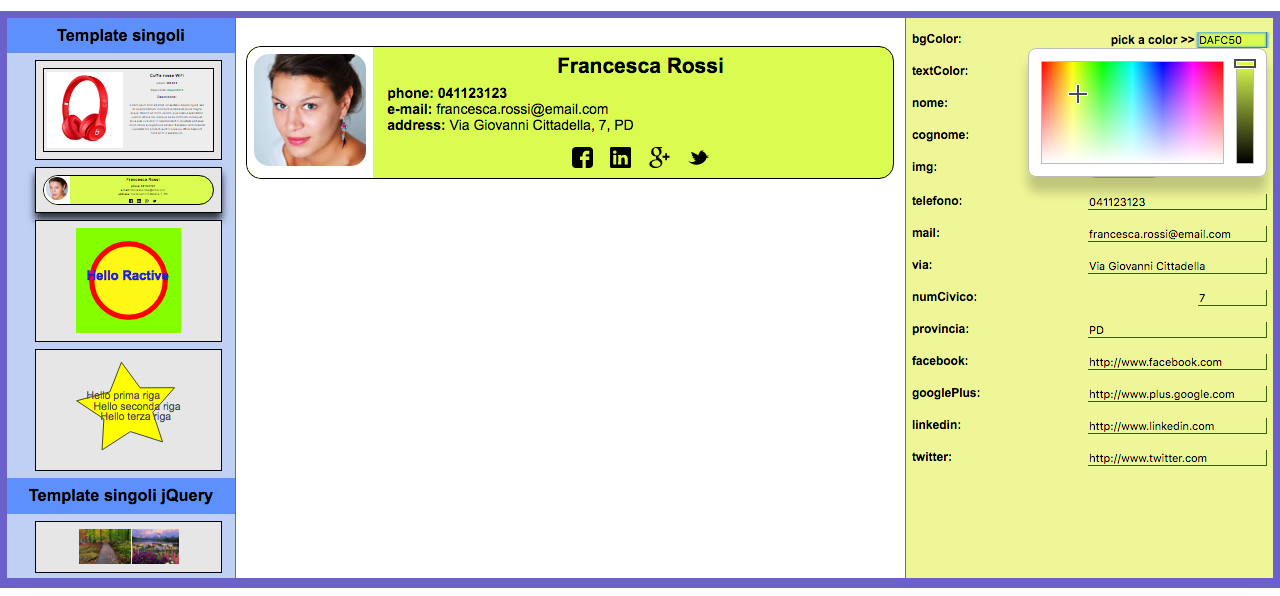
\includegraphics[scale=0.31]{../immagini/screenshot_app}
	\caption{Screenshot dell'applicazione realizzata.}
\end{figure}
I risultati ottenuti dallo studio delle librerie e l'applicazione realizzata soddisfano le aspettative dell'azienda.\\
La fase di prototipazione dei template, utilizzando la libreria \textit{Ractive.js}, ha messo in evidenza le potenzialità offerte da questo strumento e ha permesso all'azienda di trovare vari modi per sfruttare la libreria nello sviluppo dei loro prodotti.\\
Le richieste relative ai template sono state soddisfatte, dimostrando che è possibile creare template che si comportino in modo responsive e che integrino plug-in JQuery senza grandi sforzi da parte dello sviluppatore.\\
Il funzionamento dei template in ambito mobile è stato possibile tramite l'aggiunta del plug-in \textit{ractive-events-tap} che permette di gestire in maniera appropriata il tap su di un touchscreen.\\
Inoltre la possibilità di inserire il codice di attivazione per i plug-in JQuery all'interno della logica del template ne assicura la corretta esecuzione.\\
Per quanto riguarda i risultati ottenuti con l'applicazione, questi sono stati soddisfacenti per l'azienda, in quanto l'applicazione si comporta come era stato richiesto offrendo la possibilità di selezione e visualizzazione dei vari template e di modifica dei dati ad essi relativi.\\
Lo scopo principale dell'applicazione realizzata è stato quello di evidenziare le possibilità di integrazione della libreria \textit{Ractive.js} all'interno di un web application e di fornire un punto di partenza per lo sviluppo di un'eventuale estensione per l'applicativo aziendale \textit{Portal Studio}.
 
\subsection{Requisiti soddisfatti}
%RFF1.1.1 RFF2.1 RVF10
L'applicazione realizzata soddisfa tutti i requisiti obbligatori e desiderabili che sono stati individuati durante la fase di \textit{Analisi dei requisiti}.\\
Non sono stati soddisfatti i seguenti requisiti:
\begin{itemize}
	\item \textbf{RFF1.1.1} - La comparsa delle miniature all'interno della lista deve avvenire in modo animato;
	\item \textbf{RFF2.1} - La comparsa del template nel view-box deve avvenire in modo animato;
	\item \textbf{RVF10} - L'applicazione deve funzionare su \textit{Internet Explorer} versione 11.0 o superiore.
\end{itemize}
In totale sono stati soddisfatti 44 dei 46 requisiti funzionale e 9 dei 10 requisiti di vincolo.\\
Per quanto riguarda lo sviluppo dei template, il fatto che questi potessero essere resi responsive ed integrare plug-in JQuery possono essere considerati dei requisiti, anch'essi soddisfatti.
\section{Criticità}
L'unico problema riscontrato durante lo sviluppo dei template e dell'applicazione è quello relativo al caricamento \textit{on-demand} delle librerie JQuery.\\
Questo problema viene spiegato in dettaglio nella sezione \ref{subsec: problemi_lib}, esso è legato al funzionamento del \textit{browser} e alla mancanza di strumenti, offerti dallo standard, per controllare l'avvenuto caricamento delle librerie.\\
Il problema può essere risolto tramite qualche escamotage o dall'impiego di framework come \textbf{Microsoft Ajax Loader}, il cui utilizzo non era previsto durante il progetto.\\
Un altro problema incontrato è relativo al comportamento del browser \textit{Internet Explorer}, che non visualizzava in maniera corretta i template SVG.\\
Questo fatto è risultato poco importante per l'azienda che considera \textit{Internet Explorer} ormai obsoleto dopo l'avvento di \textit{Microsoft Edge}.\\
Escludendo questi due problemi, non sono emersi altre criticità durante lo svolgimento del progetto.
 
\section{Conoscenze acquisite}
Durante il periodo di stage sono state acquisite conoscenze sui \textit{template engine} e i loro possibili ambiti di utilizzo.\\
Le librerie analizzate durante il progetto erano sconosciute all'inizio dello stage, mentre a progetto terminato è stata ottenuta una discreta padronanza di esse ed in particolare della libreria \textit{Ractive.js} che, essendo stata utilizzata durante tutto il progetto, ha richiesto uno studio più approfondito.\\
Inoltre sono state affinate le conoscenze riguardanti i linguaggi per il web, in particolare JavaScript, che era già conosciuto prima dello stage, ma del quale erano sconosciuti vari aspetti come per esempio le \textit{promise}.\\
Sono state acquisite inoltre competenze a riguardo del tool di sviluppo proposto da \textit{Google}, su come utilizzare il debuger e come ottenere informazioni riguardanti i tempi di caricamento delle risorse e di rendering.\\
Lo stage ha reso possibile l'acquisizione di conoscenze relative all'ambito aziendale, dandomi la possibilità di osservare come vengono valutate le caratteristiche delle tecnologie che si ritengono promettenti per lo sviluppo di nuove soluzioni o per l'integrazione in quelle esistenti.\\
\'E stato inoltre possibile acquisire nozioni sull'organizzazione e sulle varie fasi del ciclo di vita del software, inoltre è stato possibile osservare le dinamiche aziendali e come si relaziona un team in ambito lavorativo.
 %Conclusioni

%\appendix                               
%\chapter{Gitflow}

Gitflow è un modello di sviluppo basato su Git, ideato da Vincent Driessen e presentato nel 2010 in un suo celebre post.\footnote{\url{http://nvie.com/posts/a-successful-git-branching-model/}}. Sebbene sia pittosto complicato rispetto ad altri modelli, questo framework fornisce un robusto strumento per la gestione di progetti di grandi dimensioni.

Gitflow assegna ruoli specifici ai diversi branch, specificando quando e come essi debbano interagire tra di loro. Essendo basato su Git gli sviluppatori lavorano in locale e periodicamente effettuano \textit{push} sul repository remoto centrale.

\section{I branch principali}

Nel repository principale si distinguono due rami principali:

\begin{itemize}

\item \textbf{master}, il ramo principale all'interno del quale risiede codice verificato e pronto per essere spedito in \textit{production} e in particolare tutti i suoi nodi corrispondono a \textbf{release} del prodotto, ovvero ad una versione stabile, che può essere marcata o meno con un \textit{tag};

\item \textbf{develop}, il ramo all'interno del quale avviene lo sviluppo vero e proprio del prodotto e dal quale il codice può essere rilasciato, effettuando dunque un \textit{merge} con il ramo master

\end{itemize}

\section{I branch di supporto}

Al livello inferiore dei branch principali troviamo i branch di supporto, che assistono gli sviluppatori nelle operazioni quotidiane di sviluppo. Questi branch, a differenza dei due principali, hanno un tempo di vita limitato e vengono uniti nei rami principali o semplicemente scartati. I tre branch di supporto sono:

\begin{itemize}

\item \textbf{Feature}, che viene creato dal ramo \texttt{develop} ed unito solamente nel medesimo; la loro utilità, come dice la parola stessa, è quella di creare un ramo di sviluppo per un nuovo componente del sistema. Essi normalmente vanno tenuti in locale e non devono essere \textit{pushati} sul repository remoto;

\item \textbf{Release}, che viene creato dal ramo \texttt{develop} ed unito sia nel medesimo che successivamente su \texttt{master}. Questo branch identifica le procedure che vengono istanziate all'atto della release. Quando uno sviluppatore decide di effettuare una release del prodotto apre innanzitutto un brach da \texttt{develop} chiamato \texttt{release-*}, esegue tutte le operazioni di \textit{pre-release}, effettua il merge su \texttt{develop} ed infine il merge su \texttt{master}, marcando il nodo di merge eventualmente con un \textit{tag};

\item \textbf{Hotfix}, che viene creato dal ramo \texttt{master} ed unito prima sia nel medesimo che successivamente su \texttt{develop}. Questi rami derivano dall'immediata necessità di risolvere un \textit{bug} inserito all'interno del ramo master, senza dover effettuare una nuova release. 

\end{itemize}

\begin{figure}[htp]
\centering
\includegraphics[width=\textwidth/2]{../immagini/git-flow-model}
\caption{Modello Gitflow}
\end{figure}


             % Appendice A

%**************************************************************
% Materiale finale
%**************************************************************
\backmatter
\printglossaries
% !TEX encoding = UTF-8
% !TEX TS-program = pdflatex
% !TEX root = ../tesi.tex
% !TEX spellcheck = it-IT

%**************************************************************
% Bibliografia
%**************************************************************

\nocite{*}
\printbibliography

%\bibbycategory % equivale a dare un \printbibliography per ogni categoria


\end{document}